%% 
%% Copyright 2007, 2008, 2009 Elsevier Ltd
%% 
%% This file is part of the 'Elsarticle Bundle'.
%% ---------------------------------------------
%% 
%% It may be distributed under the conditions of the LaTeX Project Public
%% License, either version 1.2 of this license or (at your option) any
%% later version.  The latest version of this license is in
%%    http://www.latex-project.org/lppl.txt
%% and version 1.2 or later is part of all distributions of LaTeX
%% version 1999/12/01 or later.
%% 
%% The list of all files belonging to the 'Elsarticle Bundle' is
%% given in the file `manifest.txt'.
%% 
%% Template article for Elsevier's document class `elsarticle'
%% with harvard style bibliographic references
%% SP 2008/03/01

\documentclass[preprint,12pt]{elsarticle}
% \documentclass{elsarticle}
%\documentclass[3p,12pt,authoryear]{elsarticle}

%% Use the option review to obtain double line spacing
%% \documentclass[authoryear,preprint,review,12pt]{elsarticle}

%% Use the options 1p,twocolumn; 3p; 3p,twocolumn; 5p; or 5p,twocolumn
%% for a journal layout:
%% \documentclass[final,1p,times,authoryear]{elsarticle}
%% \documentclass[final,1p,times,twocolumn,authoryear]{elsarticle}
%% \documentclass[final,3p,times,authoryear]{elsarticle}
%% \documentclass[final,3p,times,twocolumn,authoryear]{elsarticle}
%% \documentclass[final,5p,times,authoryear]{elsarticle}
%% \documentclass[final,5p,times,twocolumn,authoryear]{elsarticle}

\usepackage{hyperref}
\hypersetup{
  colorlinks   = true, %Colours links instead of ugly boxes
  urlcolor     = blue, %Colour for external hyperlinks
  linkcolor    = blue, %Colour of internal links
  citecolor   = red %Colour of citations
}

%% For including figures, graphicx.sty has been loaded in
%% elsarticle.cls. If you prefer to use the old commands
%% please give \usepackage{epsfig}
\usepackage{subfig}

%tables
\usepackage{booktabs}

%% The amssymb package provides various useful mathematical symbols
\usepackage{amssymb}
\usepackage{amsmath}
\usepackage{esint}

%% The amsthm package provides extended theorem environments
%% \usepackage{amsthm}

%% The lineno packages adds line numbers. Start line numbering with
%% \begin{linenumbers}, end it with \end{linenumbers}. Or switch it on
%% for the whole article with \linenumbers.
%% \usepackage{lineno}

% just for our notes
\usepackage[usenames,dvipsnames]{color}   %colors


\journal{Applied Mathematics and Computation}

%commands:
\newcommand{\defref}[1]{\hyperref[#1]{Def.~\ref{#1}}}
\newcommand{\prob}[1]{Problem~{#1}}
\newcommand{\fig}[1]{\hyperref[#1]{Fig.\ref{#1}}}
\newcommand{\figpath}{../graphics/}

%math:
\def\vc#1{\mathbf{\boldsymbol{#1}}}     % vector
\def\abs#1{\left|#1\right|}
\def\avg#1{\langle#1\rangle}
\def\d{\mathrm{d}}
\def\norm#1{\| #1 \|}
\def\abs#1{| #1 |}
\def\prtl{\partial}
\newcommand{\dd}{\; \mathrm{d}}
\newcommand{\R}{\mathbf{R}}
\newcommand{\bx}{\vc{x}}
\newcommand*\rfrac[2]{{}^{#1}\!/_{#2}}


\newcommand{\noteJB}[1]{{\color{Blue} \textbf{JB: } \textit{#1}}}
\newcommand{\notePE}[1]{{\color{Orange} \textbf{PE: } \textit{#1}}}

\newdefinition{mdef}{Definition}%[section]

\begin{document}

\begin{frontmatter}

%% Title, authors and addresses

%% use the tnoteref command within \title for footnotes;
%% use the tnotetext command for theassociated footnote;
%% use the fnref command within \author or \address for footnotes;
%% use the fntext command for theassociated footnote;
%% use the corref command within \author for corresponding author footnotes;
%% use the cortext command for theassociated footnote;
%% use the ead command for the email address,
%% and the form \ead[url] for the home page:
%% \title{Title\tnoteref{label1}}
%% \tnotetext[label1]{}
%% \author{Name\corref{cor1}\fnref{label2}}
%% \ead{email address}
%% \ead[url]{home page}
%% \fntext[label2]{}
%% \cortext[cor1]{}
%% \address{Address\fnref{label3}}
%% \fntext[label3]{}

\title{Partition of unity methods for approximation of point water sources in~porous media}

%% use optional labels to link authors explicitly to addresses:
%% \author[label1,label2]{}
%% \address[label1]{}
%% \address[label2]{}

\author[adr]{Pavel Exner\corref{cor1}}
\ead{pavel.exner@tul.cz}
\ead[url]{https://github.com/Paulie14/xfem\_project}
\cortext[cor1]{Corresponding author.}

\author[adr]{Jan B{\v r}ezina}
\ead{jan.brezina@tul.cz}

\address[adr]{Technical University of Liberec, Studentsk{\' a} 1402/2, 461 17 Liberec 1, Czech Republic}


\begin{abstract}
%% Text of abstract
In this work we demonstrate the usage of Partition of Unity (PU) methods to improve approximation of singularities 
in the solution of the Poisson equation. Our model describes a steady flow of water in a system of aquifers
which consist of porous media. The aquifers are perforated by wells and boreholes which are often represented
as point sources considering their small diameter in comparison with the vast size of the aquifer. This 
brings singularities into the solution. The extended and stable generalized finite element method 
(XFEM and SGFEM) were implemented to solve the problem and a proper adaptive integration strategy was 
developed to gain optimal convergence rates.

Several partition of unity methods (PUM) are compared on the problem of steady water flow in an aquifer-well system. 
In order to improve approximation of singularities near wells, the standard finite element space is enriched with
an analytical solution to a Laplace problem with point source on the whole $\R^2$ space. The optimal order of 
convergence in terms of $L^2$ norm of the error is demonstrated for PUM. The influence of adaptive quadrature 
and choice of enrichment domain is analysed. New strategy for adaptive integration is proposed and impact of enrichment 
radius on the error is demonstrated numerically.
\end{abstract}

\begin{keyword}
%% keywords here, in the form: keyword \sep keyword
Extended finite element method \sep 
Groundwater flow \sep
Adaptive integration \sep 
Singular solution 

%% PACS codes here, in the form: \PACS code \sep code
\PACS 02.60.Lj \sep        %Ordinary and partial differential equations; boundary value problems
\PACS 02.60.Jh             %Numerical differentiation and integration

%% MSC codes here, in the form: \MSC code \sep code
%% or \MSC[2008] code \sep code (2000 is the default)
\MSC[2010] 65N30 \sep %    Finite elements, Rayleigh-Ritz and Galerkin methods, finite methods
\MSC[2010] 35J05  %    Laplacian operator, reduced wave equation (Helmholtz equation), Poisson equation

\end{keyword}

\end{frontmatter}

%% \linenumbers

%% main text
\section{Introduction}
\label{sec:introduction}

Large scale mathematical models of the groundwater flow has to deal with the presence of small scale features like wells 
and fractures that has significant impact on the whole solution. The standard finite element method can 
capture these features using $h$ and/or $p$ adaptivity techniques 
which is payed of by greater number of degrees of freedom. One possible alternative is usage of 
suitable partition of unity method (PUM) also known as extended finite element method (XFEM). The idea is to 
augment the basis $\{\phi_n\}$ of the discrete finite element space with the functions $u_s \phi_n$, where $u_s$ is 
an a priori known solution in the vicinity of the small scale feature. 

In this work we use PUM on a steady two-dimensional aquifer model containing hydro-geological wells which
cause singularities in the solution. We follow the work \cite{gracie_modelling_2010, craig_using_2011} due to Gracie and Craig,
which up to our best knolwedge, is the first work using XFEM for the well problems.
Our primary aim is to compare different PU methods on the similar model. In particular, we use the XFEM 
and its corrected version (including ramp function and shift), e.g. by Fries in~\cite{fries_corrected_2008}, 
and the SGFEM introduced by Babu{\v s}ka and Banerjee in \cite{babuska_stable_2012, gupta_stable_2013}. We measure 
the convergence of pressure head in $L^2$ norm over the aquifer domain and we compare the used methods. 
We also investigate the error of the adaptive integration on the enriched elements and proposed more robust adaptive strategy.
In addition, we suggest better choice of enrichment area based on a tolerance criterion.

The implementation was done in C++ language using the Deal II~\cite{bangerth_deal.ii_2007}, the finite element library.
which does not support any enrichment techniques at the moment.

The paper is organized as follows. The model and its weak formulation are introduced in Section \ref{sec:model}.
In Section \ref{sec:discretization}, discretization using different partition of unity methods are presented in detail.
Analysis of the quadrature error and rules for a robust adaptive strategy are derived in In Section \ref{sec:integration}.
Section \ref{sec:enrichemnt_radius} discuss optimal choice of the enrichment area.
Section \ref{sec:results} specify data of the test problem and discuss numerical results
in particular validation of convergence, behavior of the condition number a set of experiments validating some of the theoretical results and convergence tests.
Finally, conclusions and open questions are summarized in Section \ref{sec:summary}.

\section{Model}
\label{sec:model}
We consider a steady flow in a system of aquifers (2D horizontal layers of given thickness) which are separated by 
impermeable layers (aquitards). The aquifers are connected by wells which act as sources
or sinks in the domain of each aquifer. The pressure in the aquifers is further governed by a Dirichlet boundary 
condition on the outer boundary of every aquifer.

\subsection{Mathematical model}
%We describe the wells as interior boundary condition therefore we need to define the computational domain
%as the aquifer domain with wells cross-sections cut off. 
Let $\Theta^m$ be the domain of the $m$-th aquifer,
$m=1,\ldots M$, and $z_m$ be its vertical coordinate. The well $w\in\mathcal{W}=\{1,\ldots,W\}$ is represented by an infinite vertical cylinder $B_w$
with center $\vc{x}_w$ and radius $\rho_w$.  We further denote 
\[
 B^m_w = B_w \cap \Theta^m, \quad \text{and} \quad
 B^m=\bigcup\limits_{w\in \mathcal{W}}B^m_w,
\]
for any aquifer $m$ and well $w$.
We can then define a domain $\Omega^m = \Theta^m\setminus B^m$ with an exterior boundary 
consisting of exclusive parts $\partial\Theta^m=\Gamma^m_D\cup\Gamma^m_N$ and an interior boundary 
$\partial B^m=\bigcup\limits_{w}\partial B^m_w$, 
such that $\partial\Omega^m=\partial\Theta^m\cup\partial B^m$.

The distribution of pressure head in the $m$-th aquifer is described by Poisson equation and 
boundary conditions
\begin{eqnarray} \label{eqn:poisson}
\nabla\cdot(-\mathbf{T}^m\nabla h^m) &=& f^m \qquad \textrm{on } \Omega^m\subset\R^2,\; \forall m=1,\dots,M, \\
h^m|_{\Gamma^m_D} &=& h^m_D, \\
\left(-\mathbf{T}^m\nabla h^m\cdot\vc{n}\right)|_{\Gamma^m_N} &=& 0, \\
\left(-\mathbf{T}^m\nabla h^m\cdot\vc{n}\right)|_{\partial B^m_w} &=& q^m_w \qquad \forall w\in\mathcal{W},
\end{eqnarray}
where $\mathbf{T}^m\, [\textrm{m}^2\textrm{s}^{-1}]$ denotes the transmisivity tensor,
%(we will further consider only scalar $T^m$ for simplicity), 
$h^m\, [\textrm{m}]$ the pressure head, $f^m\, [\textrm{m}\textrm{s}^{-1}]$ source density,
$\vc{n}$ unit normal vector on the boundary and
$q^m_w = Q^m_w/|\partial B^m_w|$ is the density of the flow from the well to the aquifer over the well boundary 
$\partial B^m_w$. Equation \eqref{eqn:poisson} is derived from the Darcy law and the continuity equation 
for incompressible fluid.

Presuming the aquitards to be fully impermeable, the communication between aquifers is possible only through 
wells. We can prescribe the flow balance equation 
\begin{eqnarray}
  Q^m_w &=& Q^m_{w,in} - Q^m_{w,out}, \textrm{ where} \label{eqn:well_flows} \\
  Q^m_w &\ldots& \textrm{flow into aquifer across the well boundary,} \nonumber\\
  Q^m_{w,in} &\ldots& \textrm{flow from upper aquifer,} \nonumber\\
  Q^m_{w,out} &\ldots& \textrm{flow into lower aquifer.} \nonumber
\end{eqnarray}
\begin{figure}[!htb]
  %\vspace{-15pt}
  %TODO: add arrow (flow) to the top
  \begin{center}         
    \def\svgwidth{0.5\textwidth}
    \input{\figpath well_communcation.pdf_tex}
  \end{center}
  \caption{Flow balance in the well.}
  \label{fig:well_flows}
\end{figure}

\fig{fig:well_flows} presents the equation \eqref{eqn:well_flows} and denotes the flows $Q^m_{w,\cdot}$ by red arrows.
We can look at the flows in the balance equation as 1D problems which are governed by a difference of pressure
head and a transition coefficient. Using this idea, we can substitute the flows in the equation 
\eqref{eqn:well_flows} and get
\begin{eqnarray} 
\int_{\partial B_w^m}\sigma_w^m \left(h^m - H_w^m\right) \dd s
  = c_w^{m+1}\left( H^m_w-H_w^{m+1}\right) - c^m_w\left( H^{m-1}_w-H^m_w \right), \label{eqn:well_balance} \\
 \forall m=1,\dots,M \textrm{ and } \forall w\in\mathcal{W}, \nonumber
\end{eqnarray}
where $\sigma^m_w\, [\textrm{m}\textrm{s}^{-1}]$ denotes the permeability coefficient between $w$-th well and 
$m$-th aquifer, $H_w^m$ the pressure head in the well $w$ at the level of $m$-th aquifer and finally 
$c^m_w\, [\textrm{m}^2\textrm{s}^{-1}]$ is the permeability of the well $w$ through aquitard $m$.

The problem is now to find set of functions $h^m\in C^2(\Omega^m)\cap{C}^1(\bar\Omega^m)$ and set of pressure 
values in the wells $H^m_w\in\R$, for all $m\in\{1,\ldots,M\}$ and $w\in\mathcal{W}$ that
satisfy the equations \eqref{eqn:poisson} and \eqref{eqn:well_balance}.

Note that if the lower end of well is considered isolated from below, the coefficient must be set $c^1_w = 0$.
The values of pressure head at the top of the wells $H^{M+1}_w$ are to be set on input. It is also possible
to formulate additional equations
\begin{equation} \label{eqn:well_balance_top}
  c^M_w\left( H^{M}_w-H^{M+1}_w \right) = 0,
\end{equation}
to be able to set $H^{M+1}_w$ as unknowns, but we shall leave it simple at the moment.
%With $c^m_w = 0$ we can also simulate the end of the well $w$ at the level of aquifer $m$.

% We mention yet the equation \eqref{eqn:well_balance} for $m=M+1$ which is one level above the up most aquifer
% and is adjusted to the form
% \begin{equation} \label{eqn:well_balance_top}
%   c^M_w\left( H^{M}_w-H^{M+1}_w \right) = 0.
% \end{equation}
% The pressure at the top of the well $H^{M+1}_w$ can be set as an input value or, if not set, is gained 
% as part of the solution from the equation \eqref{eqn:well_balance_top}, an example of $H^4$ in \fig{fig:well_flows}.

% The boundary term in \eqref{eqn:well_balance} with large $\sigma^m_w$ would force the pressure head along the 
% well edge to be constant (equal $H^m_w$), which cannot be in general satisfied. Therefore it is weakened and 
% later replaced by the average
% \begin{equation} \label{eqn:average}
%   \avg{h^m} = \frac{1}{\abs{\partial B^m_w}} \int\limits_{\partial B^m_w} h^m \dd s,
% \end{equation}
% which corresponds to \cite{gracie}. We use 200 points around the well edge for averaging but even smaller 
% amount is possible since our test cases are symmetric.

\subsection{Weak formulation}
We define the trial and the test spaces
\begin{eqnarray} \label{eqn:spaces}
  V &=& \prod\limits_{m=1}^{M}\big(H^1(\Omega^m)\times\R^W\big), \\
  V_0 &=& \prod\limits_{m=1}^{M}\big(H^1_0(\Omega^m)\times\R^W\big),
\end{eqnarray}
where $H^1$ and $H^1_0$ are standard Sobolev spaces and 
\[ H^1_0(\Omega^m)=\{\varphi\in H^1(\Omega^m); \varphi|_{\Gamma^m_D}=0\}. \]
We can now introduce the weak solution $u$ and test functions $v$
\begin{eqnarray} \label{eqn:solution}
   u &=& (h^1,\ldots, h^M, H^1_1,\ldots,H^{M}_W)\in V, \\
   v &=& (\varphi^1,\ldots, \varphi^M, \Phi^1_1,\ldots,\Phi^{M}_W)\in V_0.
\end{eqnarray}

To obtain the weak form we apply the standard Galerkin method. We multiply the equations \eqref{eqn:poisson} 
by test functions $\varphi^m$ and integrate by parts over $\Omega^m$, for all $m=1,\ldots,M$, to get
\begin{equation} \label{eqn:weak_form1}
  \int \limits_{\Omega^m} T^m \nabla h^m \cdot \nabla \varphi^m \dd\bx
  + \sum \limits_{w\in \mathcal{W}} \int \limits_{B^m_w} \sigma^m_w (h^m - H_w^m) \varphi^m \dd\bx
  = \int \limits_{\Omega^m} f^m\varphi^m% - \int \limits_{\Omega^m} T^m \nabla h^m_D \nabla v^m \dd\mathbf{x},
\end{equation}
% We then multiply \eqref{eqn:well_balance} by $\Phi^m_w$, subtract it from \eqref{eqn:weak_form1} 
% which results in
% \begin{multline} \label{eqn:weak_form}
%   \int \limits_{\Omega^m} T^m \nabla h^m \cdot \nabla \varphi^m \dd\bx
%         + \sum \limits_{w\in \mathcal{W}} \sigma^m_w\left( \avg{h^m}-H^m_w\right)
%           \left(\avg{\varphi^m}-\Phi^m_w\right) + \\
%           + \sum\limits_{w\in\mathcal{W}} \Big[
%           c_w^{m+1}\left( H^m_w-H_w^{m+1}\right)\Phi^m_w - c^m_w\left( H^{m-1}_w-H^m_w \right)\Phi^m_w \Big]= \\
%   =\int \limits_{\Omega^m} f^m\varphi^m \dd\bx \quad \forall m=1,\ldots,M.
% \end{multline}
% \noteJB{Consider sum over aquifers to get square term from communication on wells.
% Boundary conditions on wells?}
We then multiply \eqref{eqn:well_balance} by $\Phi^m_w$, subtract it from \eqref{eqn:weak_form1} 
and sum up over $m$ which results in
\begin{multline} \label{eqn:weak_form}
  \sum \limits_{m=1}^M \; \int \limits_{\Omega^m} T^m \nabla h^m \cdot \nabla \varphi^m \dd\bx
        + \sum \limits_{m=1}^M \sum \limits_{w\in \mathcal{W}} \; \int \limits_{\partial B^m_w} \sigma^m_w\left(h^m-H^m_w\right)
          \left(\varphi^m-\Phi^m_w\right) \dd\bx + \\
          + \sum \limits_{m=1}^M \sum\limits_{w\in\mathcal{W}}
          c_w^{m}\left( H^{m-1}_w-H_w^{m}\right)\left(\Phi^{m-1}_w - \Phi^m_w\right) 
          + \sum\limits_{w\in\mathcal{W}} c^{M+1}_w H^{M}_w \Phi^M_w = \\
  = \sum \limits_{m=1}^M \; \int \limits_{\Omega^m} f^m\varphi^m \dd\bx +
   \sum\limits_{w\in\mathcal{W}} c^{M+1}_w H^{M+1}_w \Phi^M_w \quad \forall m=1,\ldots,M.
\end{multline}
% \noteJB{Consider sum over aquifers to get square term from communication on wells.
% Boundary conditions on wells?}
We can see in \eqref{eqn:weak_form} the elliptic character of the weak form. In fact, it is possible to proove
the existence and the uniqueness using the Lax Milgram lemma. It is sufficient to have only one well pressure value 
set on input so the unique solution exists. In that case, the Neumann boundary condition can be along the 
whole outer boundary and uniqueness is still provided.

% Denoting $a^m(\cdot, \cdot)$ a bilinear form 
% \begin{equation} \label{eqn:bilinear_form_a}
%   a^m(u,v) = \int \limits_{\Omega^m} T^m \nabla u \cdot \nabla v \dd\bx
%         + \sum \limits_{w\in \mathcal{W}} \int \limits_{B^m_w} \sigma^m_w u v \dd\bx,
% \end{equation}
% we can write the weak form of \eqref{eqn:poisson}
% \begin{equation}% \label{eqn:weak_form}
%   a^m(h^m,v^m) - \int_{B_w^m}\sigma_w^m H_w^m v^m \dd\bx
%   = \int \limits_{\Omega^m} f^mv^m% - \int \limits_{\Omega^m} T^m \nabla h^m_D \nabla v^m \dd\mathbf{x},
%   \quad \forall m=1,\ldots,M,
% \end{equation}
% where the functions $h^m$ and test functions $v^m$ are from standard Sobolev spaces $H^1_0(\Omega^m)$,
% considering $h^m|_{\partial\Omega^m}=0$ for simplicity.
% The unknowns $H^m_w$ in \eqref{eqn:well_balance} are constants thus we can imagine that the test functions of 
% $H^m_w$ are also constants, chosen to be equal one, and so \eqref{eqn:well_balance} is not modified.

\section{Discretization}
\label{sec:discretization}
We can now proceed to the choice of the enrichment and the discretized tsystem of equations
\eqref{eqn:weak_form}.
Let's imagine that we have only one aquifer so we can omit the upper index $m$ in this section.
In fact, it is appropriate to do so in some notations of shape functions because we do consider the same 
triangulation for every aquifer in our implementation.

\subsection{Enrichment function}
The enrichment function in general can be obtained from the knowledge of the solution character or 
from the solution of a simple local problem which will provide us the function.
In our case the simple problem is finding pressure distribution in a circular domain $\Omega$ with one well 
placed at the center. It can be easily proved that the function
%
\begin{equation} \label{eqn:solution_form}
  h = a \log(r_w)+b, %\quad \textrm{where }
\end{equation}
where $r_w$ is a distance function
\begin{equation} \label{eqn:distance}
r_w(\vc{x}) = \|\bx - \vc{x}_w\|= \sqrt{(x-x_w)^2+(y-y_w)^2},
\end{equation}
%
is the solution of a Laplace equation $-T \Delta h = 0$, just by putting the function into the equation. 
%
We see in \eqref{eqn:solution_form} the logarithmic dependence of the pressure head on the distance from 
the well. If we represented the well only by a~point, the pressure head would go to infinity while closing 
to the point (singularity $\lim \limits_{r\rightarrow 0} \log r= -\infty$). Instead, we keep in mind the
radius of the well $\rho_w$ and introduce (global) enrichment function
%
\begin{equation}
\label{eqn:enrich_func}
s_w(\bx) = 
  \begin{cases}
  \log(r_w(\bx)), & r_w > \rho_w\\
  \log(\rho_w), & r_w \le \rho_w\\
  \end{cases}.
\end{equation}
See \fig{fig:enrich_func}.
It is natural to use the same set of $s_w$ on each aquifer since they depends only on $r_w$ and the wells are 
placed at the same positions throughout the aquifers (we consider only vertical wells, perpendicular to aquifers).
%
% and its gradient
% \begin{equation} \label{eqn:xgrad_func}
% \nabla s_w(\bx) = 
%   \begin{cases}  
%     \frac{\bx - \bx_w}{r_w^2(\bx)} & r_w>R_w \\
%     0 & r_w \leq R_w
%   \end{cases}.
% \end{equation}

%\notePE{DONE: do not forget to replace the notation of the enrichment function}
\begin{figure}[!htb]
  %\vspace{-15pt}
  %TODO: do not forget to replace the notation of the enrichment function
  \begin{center}         
    \def\svgwidth{0.5\textwidth}
    \input{\figpath enrich_func.pdf_tex}
  \end{center}
  \caption{The enrichment function.}
  \label{fig:enrich_func}
\end{figure}


In contrast to global enrichment methods, the XFEM and SGFEM apply the enrichment functions only locally. Since the enrichment function is radial it is natural
to consider the enrichment zone $Z^w = B_{R^w}(\vc x_w)$ of a well $w$ given by the so called \emph{enrichment radius} $R^w$. Local enrichment methods enrich only 
nodes that are in some enrichment zone.
\noteJB{$B_R$ is used in two different meanings, either as cylinder or as the disk (ball in $R^2$).}

    
\subsection{Partition of unity methods}
\label{sec:pum_methods}
Let $N_\alpha(\bx)$, $\alpha\in\mathcal{I}=\{1,\ldots,N\}$ be the standard linear finite element shape 
functions associated with the node $\bx_\alpha$ of the triangulation. 
In the \textbf{standard XFEM}, we write the solution in the form
\begin{equation} \label{eqn:xfem_standard_form}
  h(\bx) = \sum \limits_{\alpha\in\mathcal{I}}a_\alpha N_\alpha(\bx)
    + \sum \limits_{w\in\mathcal{W}} \sum \limits_{\alpha\in\mathcal{I}^e_w} b_{\alpha w} \phi_{\alpha w}(\bx),
\end{equation}
where $a_\alpha$ are the standard FE degrees of freedom and $b_{\alpha w}$ are degrees of freedom coming from
enrichment of the well $w$. The index set $\mathcal{I}^e_w$ includes all nodes enriched by the well $w$, which
means that we have several enrichment functions and each can enrich different nodes.
The local enrichment functions $\phi_{\alpha w}$ in \eqref{eqn:xfem_standard_form} are defined
in the following way
\begin{equation} \label{eqn:xfem_enrich}
    \phi_{\alpha w} = N_\alpha(\bx)L_{\alpha w}(\bx), \quad \alpha\in\mathcal{I}^e_w, w\in\mathcal{W},
\end{equation}
where simply the enrichment function $L_{\alpha w}(\bx) = s_w(\bx)$.

\subsubsection{Corrected XFEM}
The corrected XFEM, introduced in  \cite{fries_corrected_2008}, deals with the convergence problem on blending elements and 
introduces the \textbf{ramp function}
%\begin{equation} \label{eqn:ramp_function}
\begin{eqnarray} \label{eqn:ramp_function}
  G_w(\bx) &=& \sum \limits_{\alpha\in\mathcal{I}_w^e} N_\alpha(\bx)    \\
  &=& 
  \begin{cases}
    0 & \textrm{ on unenriched elements}    \\
    1 & \textrm{ on elements where all nodes are enriched}    \\
    ramp & \textrm{ on elements where some of the nodes are enriched}    \\
  \end{cases} \nonumber
%   \quad \textrm{ on } \tau, \textrm{ such that } \bx,\bx_\alpha\in\tau, \\
%   g_{\alpha w} &=&
%   \begin{cases}
%     1 & \textrm{ if } \alpha \textrm{ is enriched by } w \\
%     0 & \textrm{ otherwise. }
%   \end{cases}
\end{eqnarray}
%\end{equation}
It also extends the set of enriched nodes, denoted by $\mathcal{J}^e$, by enriching (unenriched) nodes 
on elements, where only some of the nodes are in $\mathcal{I}^e$. Thus $\mathcal{I}^e\subset\mathcal{J}^e$ 
and there are more enriched nodes.
The enrichment function changes into the form
\begin{equation} \label{eqn:xfem_ramp}
    L_{\alpha w} = G_w(\bx) s_{w}(\bx), \quad \alpha\in\mathcal{J}^e, w\in\mathcal{W}.
\end{equation}


In the same work, i.e. \cite{fries_corrected_2008}, authors further suggest the \textbf{shifted} enrichment functions in order 
to preserve the property of standard 
FE approximation at nodes $h(\bx_\alpha)=a_\alpha$; the value at the node is equal the corresponding degree
of freedom. The enrichment functions must be then zero at the nodes which is satisfied in the form
\begin{equation} \label{eqn:xfem_shift}
    L_{\alpha w} = G_w(\bx) \left[s_w(\bx) - s_w(\bx_\alpha)\right],
    \quad \alpha\in\mathcal{J}^e, w\in\mathcal{W}.
\end{equation} 
The property of the shifted formulation enables us to prescribe Dirichlet boundary condition such that
$a_\alpha = h_D(\bx_\alpha)$.

For the purpose of this article, let's call the two methods described above the \textbf{ramp function XFEM}  
and the \textbf{shifted XFEM}, as we shall reference to them later.

\subsubsection{SGFEM}
Finally we present the \textbf{SGFEM}, according to \cite{babuska_stable_2012,gupta_stable_2013}. 
The enrichment function is defined as the subtraction of the global enrichment function and its interpolation 
\begin{equation} \label{eqn:sgfem_enrich}
    L_{\alpha w} = \left[s_w(\bx) - \pi_\tau (s_w)(\bx)\right],
    \quad \textrm{ on } \tau,\; \alpha\in\mathcal{I}^e, w\in\mathcal{W}.
\end{equation} 
where the interpolation $\pi_\tau$ is built using the finite element shape functions
associated with nodes $\mathcal{I}(\tau)$ of the element $\tau$
\begin{equation} \label{eqn:sgfem_interpolation}
    \pi_\tau (s_w)(\bx) = \sum\limits_{\beta\in\mathcal{I}(\tau)} s_w(\bx_\beta) N_\beta(\bx).
    %\quad \textrm{ on } \tau,\; \alpha\in\mathcal{I}^e, w\in\mathcal{W}.
\end{equation}
Of course $\alpha\in\mathcal{I}(\tau)$ in \eqref{eqn:sgfem_enrich}.
Notice that there are no additional enriched nodes on blending elements, like in $\mathcal{J}^e$ in 
\eqref{eqn:xfem_ramp} and \eqref{eqn:xfem_shift}, and no ramp function is involved.

\noteJB{I miss explicit specification of discrete spaces.}

% \subsection{Assembly}
% Having the enrichment functions defined, the enriched nodes set and the equations discretized, we can approach
% the assembly of the linear system. The system has this block pattern 
% \begin{equation}
%   \begin{pmatrix}
%   \mathbf{E}^{M+1} &               &                     & \bar{\mathbf{F}}^{M+1}   & &&&&\\
%                    & \mathbf{K}^M  & \bar{\mathbf{R}}^M  & \bar{\mathbf{C}}^M       & &&&&\\
%                    & \mathbf{R}^M  & \mathbf{S}^M        & \bar{\mathbf{D}}^M       & &\ddots&&&\\
%   \mathbf{F}^{M+1} & \mathbf{C}^M  & \mathbf{D}^M        & \mathbf{E}^M             & &&&&\\
%   &&&& \ddots &&&& \\
%   &&&& & \mathbf{E}^2 &              &                    & \bar{\mathbf{F}}^2 \\
%   &&&\ddots& &              & \mathbf{K}^1 & \bar{\mathbf{R}}^1 & \bar{\mathbf{C}}^1 \\
%   &&&& &              & \mathbf{R}^1 & \mathbf{S}^1       & \bar{\mathbf{D}}^1 \\
%   &&&& & \mathbf{F}^2 & \mathbf{C}^1 & \mathbf{D}^1       & \mathbf{E}^1 \\
%   \end{pmatrix}
%   \begin{pmatrix}
%     \mathbf{H}^{M+1} \\
%     \mathbf{a}^{M} \\
%     \mathbf{b}^{M} \\
%     \mathbf{H}^{M} \\
%     \mathbf{\vdots} \\
%     \mathbf{H}^{2} \\
%     \mathbf{a}^{1} \\
%     \mathbf{b}^{1} \\
%     \mathbf{H}^{1} \\
%   \end{pmatrix} =
%   \begin{pmatrix}
%     \mathbf{f}^{M+1}_H \\
%     \mathbf{f}^{M}_a \\
%     \mathbf{f}^{M}_b \\
%     \mathbf{f}^{M}_H \\
%     \mathbf{\vdots} \\
%     \mathbf{f}^{2}_H \\
%     \mathbf{f}^{1}_a \\
%     \mathbf{f}^{1}_b \\
%     \mathbf{f}^{1}_H \\
%   \end{pmatrix}
% \end{equation}
% where $\mathbf{K}^m$ is the matrix of the standard FE approximation, $\mathbf{S}^m$ is the matrix of the 
% enrichment, $\mathbf{R}^m$ relates standard FE and enrichment,  $\mathbf{E}^m$ is the matrix associated with 
% unknown pressures in the wells and 
% $\mathbf{C}^m$, $\mathbf{D}^m$ and $\mathbf{F}^m$ are communication matrices: standard FE -- well, 
% enrichment -- well and well -- well, respectively. The whole system is symmetric.
% 
% The entries of the matrices are 
% 
% \begin{eqnarray}
%   K^m &=& \left[a^m(N^m_\alpha, N^m_\beta)\right]   ,\qquad \forall \alpha,\beta\in \mathcal{I} \label{eqn:k_entry}\\
%   S^m &=& \left[a^m(\phi^m_{\alpha k}, \phi^m_{\beta j})\right]     ,\qquad \forall \alpha,\beta\in \mathcal{I}^e,\; \forall k,j\in\mathcal{W} \label{eqn:s_entry}\\
%   R^m &=& \left[a^m(N^m_{\alpha}, \phi^m_{\beta j})\right]      ,\qquad \forall \alpha\in \mathcal{I},\; \forall\beta\in\mathcal{I}^e,\; \forall j\in\mathcal{W} \label{eqn:r_entry}\\
%   C^m_{w\alpha} &=&-\int\limits_{B^m_w} \sigma^m_w N^m_\alpha   ,\qquad \forall \alpha\in \mathcal{I},\; \forall w\in\mathcal{W}\\
%   D^m_{w\alpha j} &=&-\int\limits_{B^m_w} \sigma^m_w \phi^m_{\alpha j}  ,\qquad \forall \alpha\in \mathcal{I}^e,\; \forall w\in\mathcal{W}\\
%   \rm{diag}(\mathbf{E}^m)_w &=&\int\limits_{B^m_w} \sigma^m_w + c^{m+1}_w   ,\qquad \forall w\in\mathcal{W}\\
%   \rm{diag}(\mathbf{F}^m)_w &=& -c^m_w ,\qquad \forall w\in\mathcal{W}
% \end{eqnarray}


\section{Integration on enriched elements}
\label{sec:integration}
In order to compute the entries of the system matrix, %\eqref{eqn:s_entry} and \eqref{eqn:r_entry} 
we need to integrate
the expressions containing the enrichment functions. These of course can be non-polynomial, like they are 
in our case. The standard quadrature rules are not appropriate any more, for they are constructed to integrate 
precisely polynomials up to a given degree. The higher requirements on integration precision
are the price for using enrichment functions and a coarse mesh.

There are two aspects which the integration must handle properly:
\begin{itemize}
  \item the steep gradient of enrichment base functions in the vicinity of a well (the singularity),
  \item the well edge geometry, since the elements of the triangulation do not take the well into account.
\end{itemize}

Since the integrated functions can be very large near the singularity, even small changes in the domain shape 
can lead to large errors in integration.
One of the approaches to improve integration is an adaptive quadrature. This way the element is divided into 
subregions (squares on the reference element) only to place more quadrature points inside but not to bring 
any more degrees of freedom in the system. We will discuss the adaptivity criteria, suggest improvement and 
compare our solution with the original one (developed in \cite{gracie_modelling_2010}) in the following subsection. 

\subsection{Instability of adaptive quadrature}
\label{sec:refinement_element}
Gracie and Craig in \cite{gracie_modelling_2010} refine only subregions that cross the boundary of the well, using at most 12 refinements.
This catches nicely the well edge but it works only when the well is placed at the node of an element or near the center of an element. 
When the well is placed near the edge of an element, there can be
a large difference in the size of neighboring subregions, see Figure \fig{fig:adapt_ref_a}. Although
the integrand is computed precisely enough on the element with the well inside, the quadrature points on the
neighboring elements (where the integrand has still large derivatives) are placed very sparsely 
and the integration error is large.

\begin{figure}[!htb]
%   \vspace{0pt}
  \centering    
  \subfloat[refinement due to G. and C.]{\label{fig:adapt_ref_a} 
    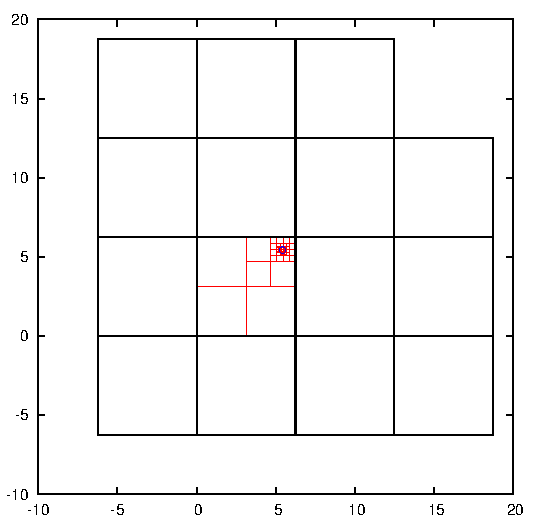
\includegraphics[width=0.45\textwidth]{results/adaptive_refinement_3_old.pdf} }
  \hspace{0pt}
  \subfloat[improved refinement]{\label{fig:adapt_ref_b} 
    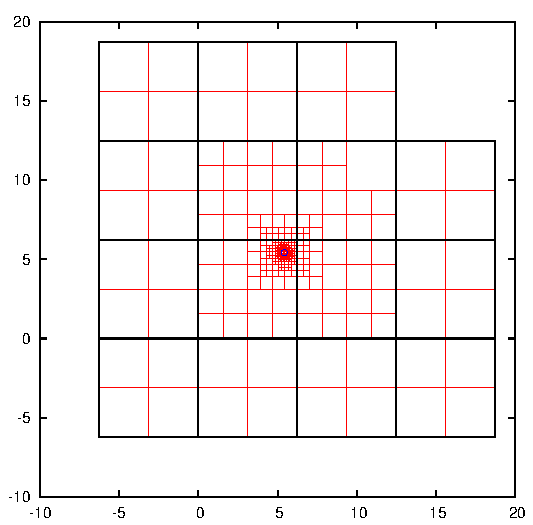
\includegraphics[width=0.45\textwidth]{results/adaptive_refinement_3_new.pdf} }
  \caption[Adaptive refinement comparison]
  {Comparison of the original and improved refinement techniques.
   Black lines denote enriched elements edges, red lines denote adaptive refinement (subregions edges) and the well
   edge is blue.
  }
  \label{fig:adapt_refinement}
\end{figure}
In order to overcome this instability of the adaptive quadrature, we have made an asymptotic analysis of the integration error presented 
in the next section.

\subsection{Estimate of quadrature error}

Let us assume only one well of radius $\rho$ situated at the origin. In the case of elliptic equation, the term with the strongest singularity is 
\begin{equation}
    \label{eq:term-of-interest}
    f(r)=(\nabla \log r )^2 \approx r^{-2}
\end{equation}
which is also the worst term to integrate independently of the particular variant of the PU method.
Consider a~subregion $S$ with a~side $\delta$ and 
let us denote $r_{S}$ the distance of $S$ to the origin.
We shall estimate the error of the 2D tensor product Gauss quadrature rule of the order $n$ ($n$ times $n$ points) on the square $S$. Let us denote 
$\Pi^n f$ the projection of an integrand to the space of polynomials that are integrated exactly. Due to the radial nature of the integrand and its derivatives,
we can estimate
\[
  \abs{f-\Pi^n f}(x,y) \le \abs{f-\Pi^n f}(x,y_0), \quad \text{for } \abs{y_0} \le \abs{y},
\]
and thus estimate the error by the error $E^n$ of 
 1D quadrature of the same order on $(r_{S}, r_{S}+\delta)$:
\[
  \int_S \abs{f-\Pi^n f} \le \delta E^n((r_{S}, r_{S}+\delta)).
\]
The error of 1D Gauss quadrature of order $n$ ($n$ quadrature points) over an interval $(r,r+\delta)$ is 
\[
  E_n = \frac{\delta^{2n+1} (n!)^4}{(2n+1)((2n)!)^3} f^{(2n)}(\xi_n) 
\]
for some $\xi_n \in (r, r+\delta)$, see e.g. \cite{kahaner_numerical_1989}. 
Regarding the integrand \eqref{eq:term-of-interest}, we have 
\[
  \abs{f^{(2n)}(r)} = (2n+2)! r^{-(2n+2)}.
\]
Finally, we get an estimate for the quadrature error on a single subregion:
\[
    \int_S \abs{f-\Pi^n f} \le  \alpha_n \left( \frac{\delta}{r_{S}} \right)^{2n+2}, 
  \qquad \alpha_n = (2n+2)\left( \frac{(n!)^2}{(2n)!} \right)^2.
\]
This estimate implies that we have to ensure $\delta < r_S$ in order to get a decent quadrature error 
and possibly to employ a higher order quadrature. 


%JB%Derived criterion holds only on squares, where the integrated function is smooth.
%JB%This is not the case for squares intersecting the boundary of the well, $r_{S} \le \rho \le r_{max}$, where we integrate 
%JB%discontinuous function $\chi_{S \setminus W} f$. Using substitution, we can map $W$ to unit circle $B$
%JB%\[
%JB%  \int_{S} \chi_{S \setminus W} \frac{1}{r^2} \d \vc r= \int_{S'} \chi_{S' \setminus B} \frac{1}{r'^2} \d \vc {r'},
%JB%\]
%JB%where $S'$ is square with side $H=\delta/\rho$ and $\vc {r'} = \vc{r}/\rho$. Empirically determined error of the midpoint rule for later 
%JB%integral is
%JB%\[
%JB%    E(H) = c_e H^{p_e}, \quad \text{with } c_e=0.08,\ p_e=2.5.
%JB%\]
%JB%This error has to be smaller then $\epsilon h^2$, thus for $h$ we get formula:
%JB%\begin{equation} \label{eqn:h_criterion}
%JB%   h\le h_b(\epsilon) = \Big(\frac{\epsilon \rho^{p_e}}{c_e}\Big)^{\frac{1}{p_e-2}}. 
%JB%\end{equation}
%JB%
%\noteJB{TODO: modify test of integration on unit disk for the function $1/r^2$.}

\subsection{A priori adaptive quadrature rules}
Let us denote $r_{min}$ the minimum and $r_{max}$ the maximum distance to the center of a well from a subregion. 
Based on the analysis presented above, we propose following adaptive quadrature rules:
%JB%\begin{enumerate}
%JB% \item If $r_{max} < \rho$ the square quadrature is zero.
%JB% \item If $r_{min} < \rho < r_{max}$ (square cross the well boundary) we subdivide the square unless $\delta < 2^{-12}h$.
%JB% \item If $r_{min} > \rho$. For $\frac{h}{r_{min}} > \frac{1}{2}$ subdivide the square, else select order $n$ so that 
%JB% \begin{equation} \label{eqn:alpha_criterion}
%JB%    \frac{\alpha_n h^{2n}}{r_{min}^{2n+2}} \le \epsilon,
%JB% \end{equation}
%JB% use at least the same order as necessary for FEM.
%JB%\end{enumerate}
%JB%
%\noteJB{TODO:
%We should estimate true error numerically using one more subdivision and compare it to prescribed tolerance, we should be safely 
%below, without increasing the number of evaluation compared to current implementation.
%}



%JB%We suggest additional criterion for subelements refinement which takes into account a subelement diameter 
%JB%and its distance from the well
%JB%\begin{equation}
%JB%  h \leq C_R r_{min},
%JB%\end{equation}
%JB%\notePE{Originally, I compute $r_{min}$ between vertices and the well center, but I believe that the results would be the same.}
%JB%where $h$ is the diameter of the subelement and $r_{min}$ is the minimal distance between a vertex of 
%JB%the subelement and the well center. $C_R$ is a scaling constant, equal 0.5 by default, through which we can 
%JB%control the significance of the criterion. If satisfied, the subelement is not refined anymore.
%JB%

%JB%Eventually, we do 10 levels of improved adaptive refinement with the following rules ($r_{max}$ is the maximal
%JB%distance of a vertex of the subelement and the well center):
\begin{enumerate}
 \item If $r_{max} < \rho$, the subregion is not refined and the quadrature is zero.
 \item If $r_{min} < \rho < r_{max}$ and $\delta > 2^{-10}h$, the subregion is refined.
 \item If $r_{min} < \rho < r_{max}$ and $\delta \le 2^{-10}h$, $3\times3$ Gauss quadrature is used.
 Values at quadrature points lying inside the well are set to zero.
 \item If $r_{min} > \rho$ and $\delta > r_{min} / 2$, the subregion is refined.
 \item If $r_{min} > \rho$ and $\delta \le r_{min} / 2$, $3\times3$ quadrature is used.
\end{enumerate}


These rules ensure $\delta < r_{min}/2$ outside the well, where the integrand is smooth. Subregions intersecting 
the well's boundary are refined using at most $10$ refinement levels, since the integrand is discontinuous there and we cannot employ 
estimates from the previous section. The maximum number of levels is chosen so that we get similar total number of quadrature points 
as in the quadrature used by G. and C. in \cite{gracie_modelling_2010}. Using the proposed rules, the elements that do not contain the well are refined as well,
see \fig{fig:adapt_ref_b}. 

Implementation of this approach allows the convergence rates of the used PU methods to close up to the optimum,
as the results of the numerical tests will show in section \ref{sec:results}.


% In \fig{fig:adapt_refinement_norm} you can see the $L_2$ norms of the error on the enriched elements.
% The first one is computed using the original adaptive quadrature where $3\times3$ quadrature rule is applied 
% on the enriched element with the well and $4\times4$ quadrature rules on the other enriched elements. 
% The improved adaptive quadrature is computed as described above. Notice the scale of the improved version -- 
% the error on elements is in small range and is not significantly concentrated anywhere. In contrast, 
% the original version shows out large error that is concentrated on the closest non-refined element to the well.
% 
% 
% \begin{figure}[!htb]
% %   \vspace{0pt}
%   \centering    
%   \subfloat[original]{\label{fig:adapt_ref_norm_a} 
%     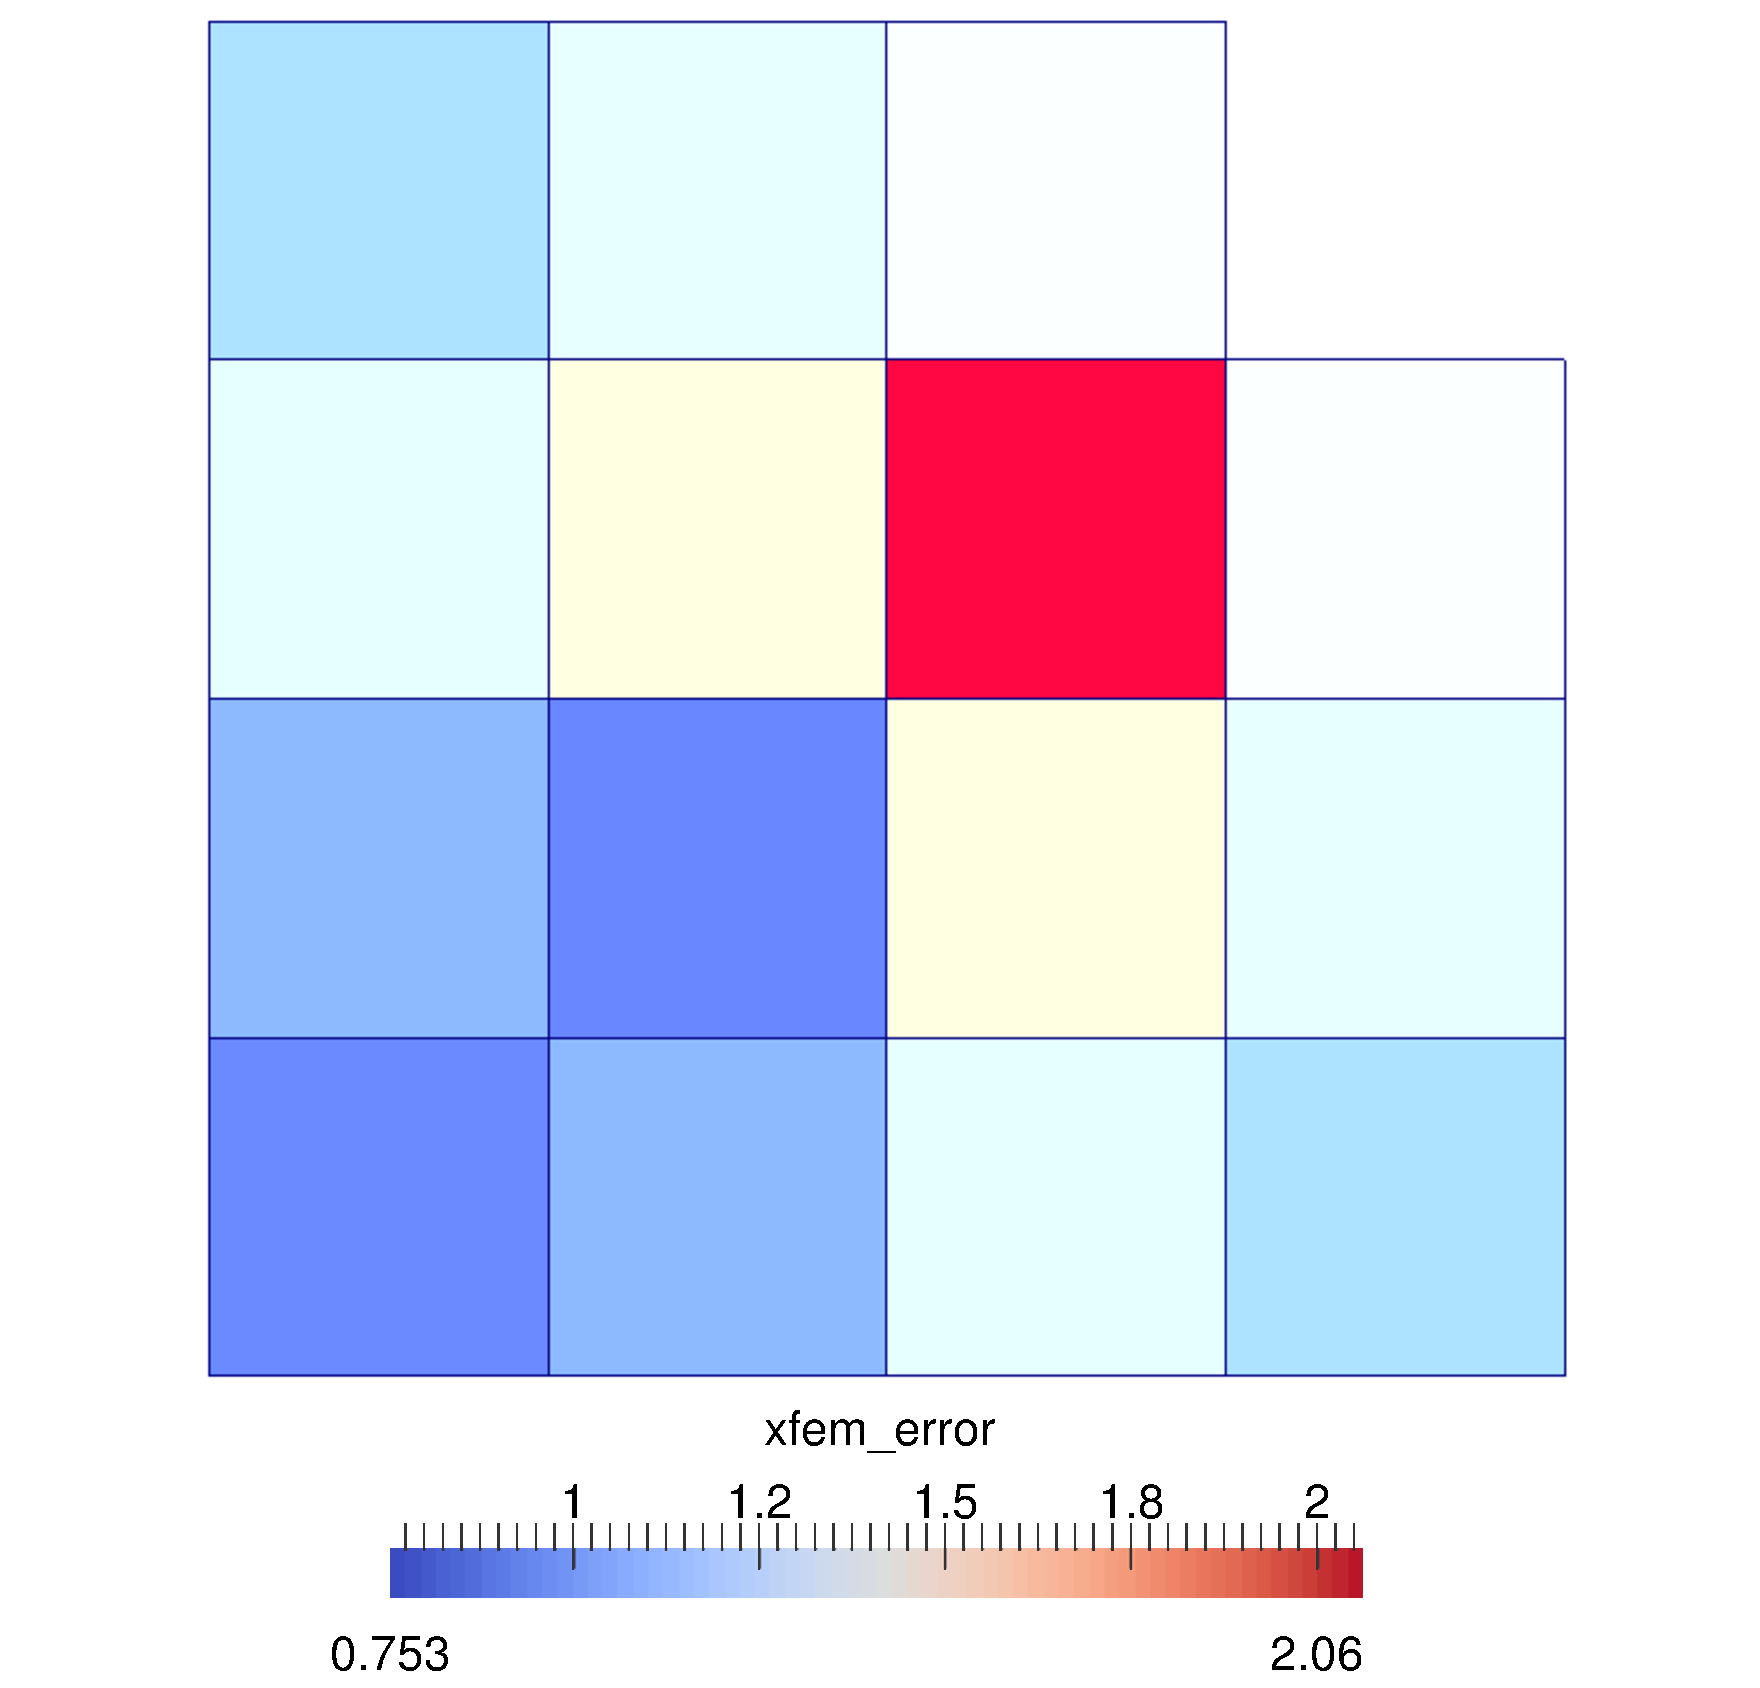
\includegraphics[width=0.45\textwidth]{results/adaptive_refinement_extract_3_old.pdf} }
%   \hspace{0pt}
%   \subfloat[improved]{\label{fig:adapt_ref_norm_b} 
%     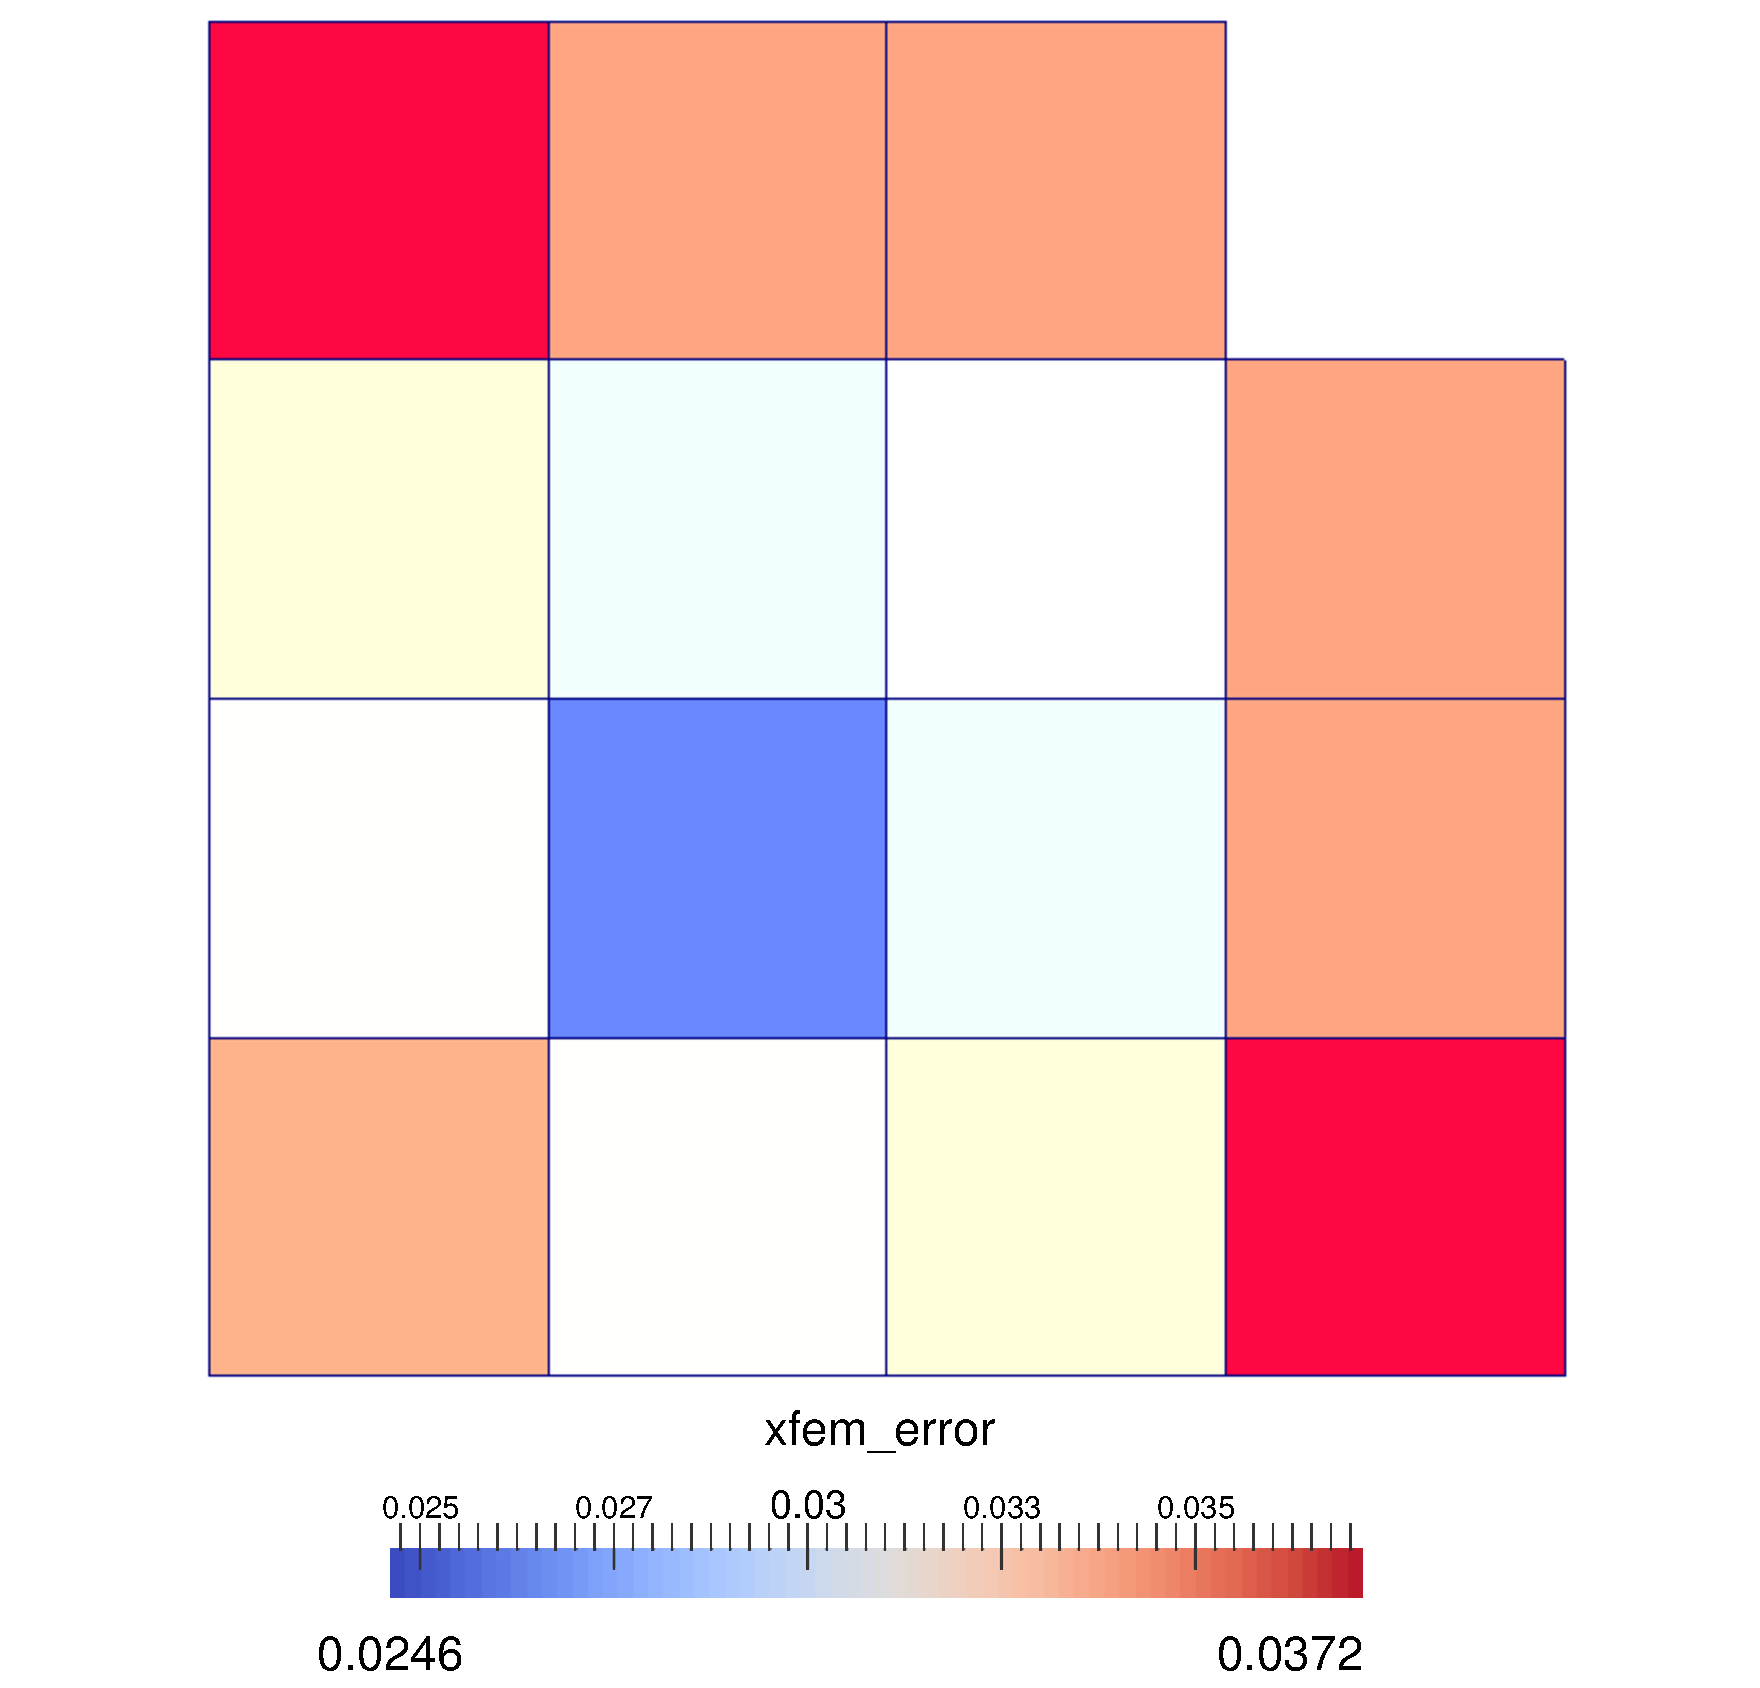
\includegraphics[width=0.45\textwidth]{results/adaptive_refinement_extract_3_new.pdf} }
%   \caption[Adaptive quadrature refinement comparison]
%   {Comparison of element-wise error in $L_2$ norm using original and improved adaptive quadrature.
%   \notePE{TODO: add axis, remove legend label, try to sharpen}
%   }
%   \label{fig:adapt_refinement_norm}
% \end{figure}

% \subsection{Circle integration experiment}
% The approximation of the integration domain is also the source of the error. We decided to run 
% an experiment on integrating the characteristic function of the well with our adaptive integration.
% The domain $\Omega$ is a square $4\times4$ out of which a circle of radius 1.0 is cut off. The characteristic 
% function is considered
% \begin{equation}
%   \chi(\bx) = \left\{
%     \begin{array}{l l}
%       0 & \quad \textrm{if } \bx \textrm{ is inside the circle}\\
%       1 & \quad \textrm{otherwise}
%   \end{array} \right.
% \end{equation}
% and the integral 
% \begin{equation}
%   \int_{\Omega}\chi(\bx) \dd\bx = 4^2 - \pi
% \end{equation}
% is equal the area of the square minus the area of the circle.
% 
% In this experiment we investigate the influence of the order of the quadrature rule and the level of
% the refinement on how precisely the well geometry is captured.
% 
% In the graph in \fig{fig:adapt_ref_convergence} we can see that for all the quadratures the convergence rate
% is similar, around 1.5. The gain from using higher order quadratures is not worth, especially in case 
% of the order 4 the error is not much smaller than the error of the quadrature of the order 3. 
% 
% Finally the highest level of refinement is chosen to be 10 and the quadrature order to be 3. The number of
% the quadrature points generated by the process described above in \ref{sec:refinement_element} is then similar 
% both in the original (14793) and improved version (14819).
% 
% \begin{figure}[!htb]
% %   \vspace{0pt}
%   \centering    
%   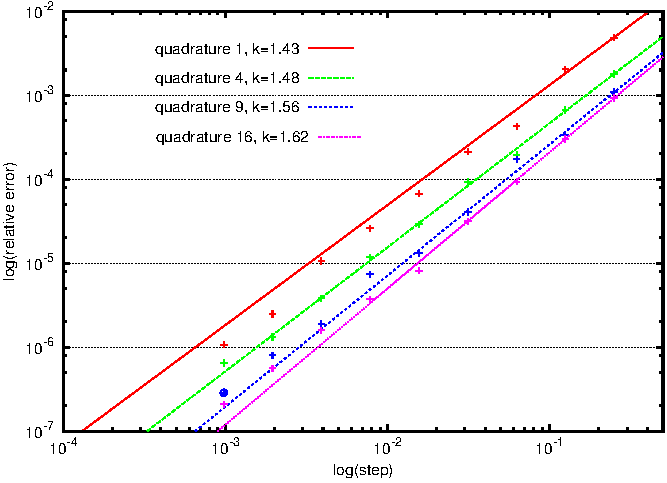
\includegraphics[width=0.7\textwidth]{results/adaptive_integration.pdf}
% %   \subfloat[rozdìlený element s vrtem]{\label{fig:adapt_ref_a} 
% %     \includegraphics[width=70mm]{\figpath adaptive_ref.pdf} }
% %   \hspace{0pt}
% %   \subfloat[detail hranice vrtu]{\label{fig:adapt_ref_b} 
% %     \includegraphics[width=72mm]{\figpath adaptive_ref_detail.pdf} }
%   \caption[Adaptive refinement convergence]{Convergence of adaptive refinement of a circle cutoff.}
%   \label{fig:adapt_ref_convergence}
% \end{figure}



%JB%\subsection{Adaptive integration experiment}
%JB%We now describe the experiment from which we obtained the coefficients in the criterion 
%JB%\eqref{eqn:h_criterion}. Let us have a single element, a square $4\times4$, out of which a circle of unit radius 
%JB%is cut off -- this represents an element with a well. We now want to investigate integration error
%JB%in the vicinity of the circle on the function $f=r^{-2}$, $r$ being the distance from the center of the circle. 
%JB%
%JB%We compute the integral on the selected level of refinement only on the squares intersecting the circle. Then
%JB%we refine the squares up to the 12-th level, integrate again and compute the difference. Quadratures rules
%JB%$1\times1$, $2\times2$, $3\times3$ and $4\times4$ are used. The results are shown in 
%JB%\fig{fig:adapt_integration_conv} also with convergence trend lines equations. The conclusion can be made
%JB%that it is more efficient to refine one more level with one-point quadrature than to use higher order 
%JB%quadrature on the coarser level. As for the coefficient, these can be read from the graph -- for the one point
%JB%quadrature $c_e=12.65$ and $p_e=1.27$.
%JB%
%JB%\begin{figure}[!htb]
%JB%%   \vspace{0pt}
%JB%  \centering    
%JB%  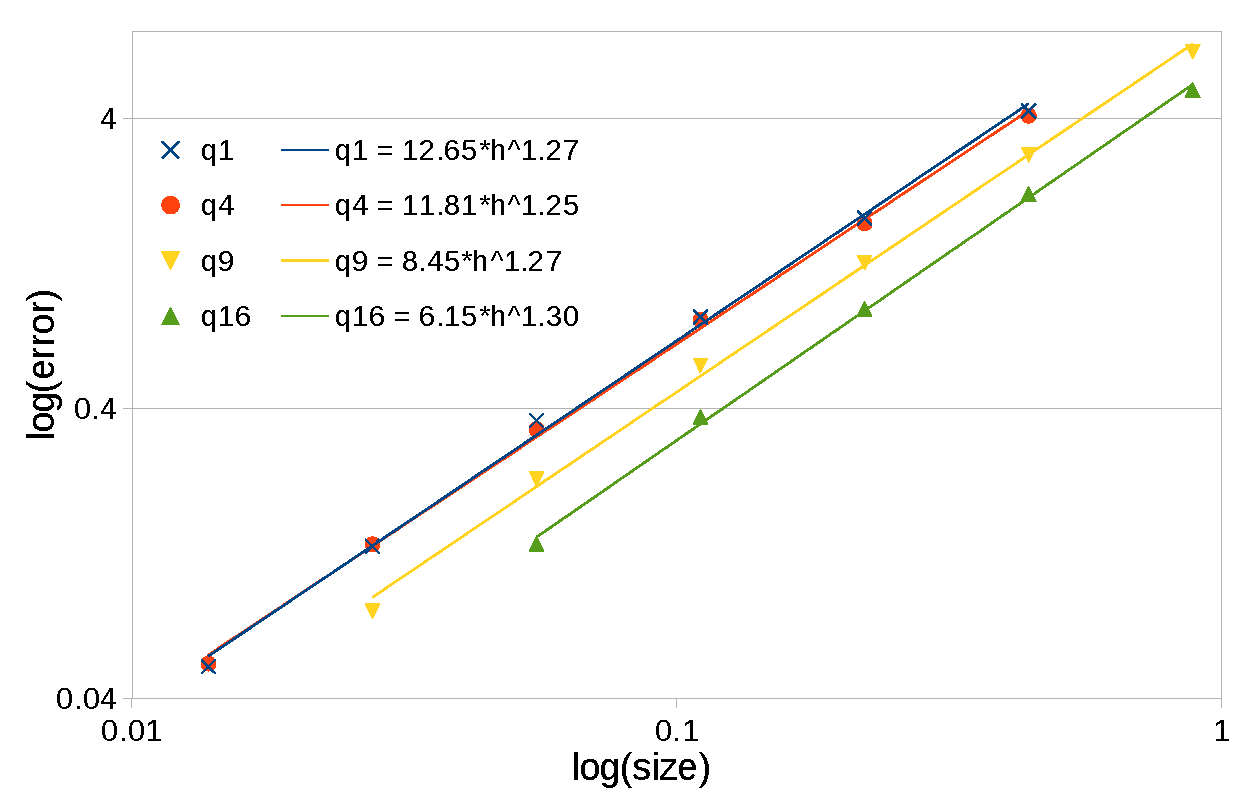
\includegraphics[width=0.9\textwidth]{results/adapt_integration_conv.pdf}
%JB%%   \subfloat[rozdìlený element s vrtem]{\label{fig:adapt_ref_a} 
%JB%%     \includegraphics[width=70mm]{\figpath adaptive_ref.pdf} }
%JB%%   \hspace{0pt}
%JB%%   \subfloat[detail hranice vrtu]{\label{fig:adapt_ref_b} 
%JB%%     \includegraphics[width=72mm]{\figpath adaptive_ref_detail.pdf} }
%JB%  \caption[Adaptive quadrature convergence.]{Convergence graph of adaptive quadrature on function $r^{-2}$.
%JB%  \\ \notePE{thicker trend lines}}
%JB%  \label{fig:adapt_integration_conv}
%JB%\end{figure}
%JB%
\section{Estimate the enrichment radius} \label{sec:enrichemnt_radius}
In this section, we shall study dependence of the solution error on the enrichment radius $R$. First part is devoted to 
theoretical analysis the later part presents numerical results.
Let us consider a general elliptic problem to find $u\in V$ satisfying
\[
   a(u, \phi) = \langle f, \phi \rangle, \text{ for } \phi \in V,
\]
where $a$ is bounded elliptic bilinear form: $\norm{a}\le M_a$, $a(v, v) \ge \gamma \norm{v}_V^2$, $\gamma>0$, and $f$ an bounded linear form, $f\in V'$. 
Suppose, that the problem is to be solved on a domain $\Omega \subset \R^2$ with a single hole (well) of radius $\rho$ at the origin. 
Let us assume, that the solution can be split to the singular part $u_s(\vc x)= \log |\vc x|$ and the regular part $u_r=u-u_s$.
Let $V^P_h$ be a polynomial finite element subspace of $V$ on a regular mesh of elements with a maximal diameter $h$
and let $V_h$ be a such enriched space that $u_s$ can be approximated exactly on the enrichment zone $Z_R$, i.e.
\[
   \inf_{v\in V_h} \norm{u_s - v}_V = \inf_{v\in V^P_h} \norm{u_s|_{Z'_R} - v}_V, \quad Z'_R = \Omega\setminus Z_R.
\]
Using standard error estimate for elliptic PDE (e.g. \cite[Theorem 13.1]{ciarlet_basic_1991}), we get
\begin{equation}
    \label{eq:std_err_estimate}
    \norm{u - u_h}_{V} \le c_a \inf_{v \in V_h} \norm{u - v}_{V} 
    \le c_a \big(\inf_{v \in V^P_h} \norm{u_r - v}_{V} + \inf_{v \in V_h} \norm{u_s - v}_{V} \big).   
\end{equation}
where $c_a=1+\norm{a}/\gamma$.
In the following, we consider $V=H^1(\Omega)$, square grid and $V^P_h$ formed by bilinear finite elements. 
Then \eqref{eq:std_err_estimate} can be further estimated using approximation property of $V^P_h$:
\begin{equation}
    \label{eq:particular_estimate}
    \norm{u - u_h}_{H^1(\Omega)} \le c_a \big(c h \abs{u_r}_{H^2(\Omega)} + \norm{u_s - \Pi u_s}_{H^1(Z'_R)} \big)   
\end{equation}
where $\Pi u_s$ denotes interpolation of $u_s$ in $V^P_h$. Our next aim is to find tight estimate for the second term.
To this end, we calculate $H^1$ error on a single square element $S_{h,r}$ with side $h$ and distance $r$ from origin.
Using parametrization $0<s,t<1$,  we get

\begin{align*}
 (u_s - \Pi u_s)(s,t)&=\log\sqrt{(r+hs)^2+(ht)^2} -\Big[(1-s)(1-t)\log r + (1-s)t\log\sqrt{r^2+h^2}\\
 &\quad+ s(1-t) \log(r+h) + st\log\sqrt{(r+h)^2+h^2} \Big]\\
 &=\frac12 \frac{h^2}{r^2}\big(t^2-t - s^2 +s\big) + O(\frac{h^3}{r^3})
\end{align*}
and 
\begin{equation}
 \nabla(u_s - \Pi u_s)(s,t) = \frac{h}{r^2} \Big( \frac12-s, t-\frac12 \Big) + O(\frac{h^2}{r^2}).
\end{equation}
Assuming $h<r$, we can neglect higher order terms. Then by direct integration
\begin{align*}
 \norm{u_s - \Pi u_s}^2_{L^2(S_{h,r})} \approx \frac14 \frac{h^6}{r^4}\int_0^1\int_0^1 (t^2-t-s^2+s)^2\,\d s\, \d t = \frac{1}{360}\frac{h^6}{r^4} 
\end{align*}
and
\begin{equation}
    \label{eq:grad_estimate_on_square}
    \norm{\nabla(u_s - \Pi u_s)}^2_{L^2(S_{h,r})} \approx \frac{2h^4}{r^4} \int_0^1 \Big(t-\frac12\Big)^2 \d t = \frac{1}{6}\frac{h^4}{r^4}.
\end{equation}
Thus for the density of squared error we have
\[
    \frac{1}{\abs{S_{h,r}}} \norm{u_s - \Pi u_s}^2_{H^1(S_{h,r})} \approx \frac{h^2}{6r^4}
\]
which after integration over the unenriched domain gives final estimate:
\begin{equation}
    \label{eq:singular_approx_error}
    \norm{u_s - \Pi u_s}_{H^1(Z'_R)} \le \left[\int_0^{2\pi} \int_R^\infty \frac{h^2} {6r^4} r \,\d r\, \d \phi\right]^{1/2} = \sqrt\frac{\pi}{6}\frac{h}{R}. 
\end{equation}

Recalling the estimate \eqref{eq:std_err_estimate}, we can conclude that optimal choice of the enrichment radius is $h/R\approx \norm{u_r-\Pi u_r}_H^1(\Omega)$, 
which balance error in the regular and the singular part. In combination with an a posteriori error analysis this could give a rule for automatic
determination of the enrichment radius.



\section{Numerical results}
\label{sec:results}

\subsection{Test problems} \label{sec:test_cases}
In this section we define problems that we solve in our numerical experiments. We restrict ourselves to 
single aquifer problems for the purpose of this article but our implementation enables multi-aquifer systems 
as well. In order to measure convergence, it is desirable to have an analytic solution which will be also derived. 

Suppose we have the following problem
\begin{equation} \label{eqn:poisson_problem}
\left.\begin{aligned}
    -T \Delta h &= TU\omega^2\sin(\omega x) \qquad \textrm{on } \Omega \\
    h|_{\partial\Omega} &= h_D\\
    \left(-T\nabla h\cdot\vc{n}\right)|_{\partial B_w} &= \sigma_w\left(h - H_w\right) \\
    \end{aligned}
    \;\right\}
\end{equation}
where the pressure head $H_w$ at the well and $h_D$ on the boundary are given. 
The domain $\Omega$ is a square with diagonal $2R$ with the well placed in the center $\vc{x}_w$.
Note that we neglected the influence of $c^2_w$ by eliminating the equation from the system (we consider 
$H_w = H^1_w = H^2_w$). We further set $c^1_w=0$ and $T=1.0$. 

We will look for the solution $h$ of \eqref{eqn:poisson_problem} in the form
\begin{equation} \label{eqn:poisson_solution}
  h=a\log\left(\frac{r_w}{R}\right)+U\sin(\omega x)
\end{equation}
which solves the Poisson equation in \eqref{eqn:poisson_problem}. 
To obtain $a$, we use the average pressure head along the well edge in the third equation 
of \eqref{eqn:poisson_problem}:
\begin{equation} \label{eqn:a_average_derivation}
    \fint \limits_{\partial B_w} -\nabla h \cdot \vc{n} = \sigma_w\left(H_w - \langle{h}\rangle \right), 
    \qquad \textrm{ where} \langle{h}\rangle = \fint \limits_{\partial B_w} h.
\end{equation}
The integral in \eqref{eqn:a_average_derivation} cannot be calculated precisely therefore it is approximated with error 
$O(\omega^2 \rho_w)$. Finally we have
\begin{equation} \label{eqn:a_constant}
    a=\frac{\rho_w \sigma_w \big[H_w - U\sin(\omega x_w) - \frac{U\omega^2}{2\sigma_w}\sin(\omega x_w)\big]}
           {\rho_w \sigma_w \log\left(\frac{\rho_w}{R}\right) - 1}.
\end{equation}
The solution \eqref{eqn:poisson_solution} is then used to define the boundary function $h_D$.

Let us now define the input data. $\Omega$ is a square $(-100,100)\times(-100,100)$ and the well is characterized by 
$\vc{x}_w=[5.43,5.43]$,  $\rho_w=0.2$, $H_w=100$ and $\sigma_w=10^5$. The \prob{1} is to find solution $h$ of
\eqref{eqn:poisson_problem} with $U=0.0$ which means that the right hand side of the Poisson equation vanishes.
The \prob{2} is to find solution $h$ of \eqref{eqn:poisson_problem} with $U=8.0$ and $\omega=0.03$.


% \begin{prob}[Laplace equation] \label{def:test_case_1}
% Find the solution $h$ of a single aquifer problem
% \begin{eqnarray*} \label{eqn:laplace_problem}
%     -T \Delta h &=& 0 \qquad \textrm{on } \Omega \\
%     h|_{\partial\Omega} &=& h_D \\
%     H_w = H^2_w &=& P_w \\
%     \left(-T\nabla h\cdot\vc{n}\right)|_{\partial B_w} &=& q_w \\
% \end{eqnarray*}
% where the pressure $P_w$ at the well and the pressure $h_D$ at the boundary are given.
% The domain $\Omega$ is a square with a single well placed near the center in $\vc{x}_w$.
% \end{prob}
% We can find the analytic solution of \probref{def:test_case_1} but on a circular disk where we have the zero 
% pressure on the outer boundary. The solution is considered in the form $h=a\log(\frac{r_w}{R})$ 
% where $R$ is the radius of the circular domain. Transmisivity is further set $T=1.0$ for simplicity.
% Now we can use the boundary condition to find the constant $a$ such that it satisfies
% \begin{eqnarray*}
%   -T\nabla h \cdot \vc{n} = \sigma_w(P_w - h),
% \end{eqnarray*}
% where $\rho_w$ is the well radius.
% The solution is then
% \begin{equation} \label{eqn:laplace_solution}
%   h=a\log\left(\frac{r_w}{R}\right) \qquad \textrm{ with } 
%     a=\frac{\rho_w \sigma_w P_w}{\rho_w \sigma_w \log\left(\frac{\rho_w}{R}\right) - 1}
% \end{equation}
% The function \eqref{eqn:laplace_solution} is just the analytic solution of \probref{def:test_case_1} when 
% \eqref{eqn:laplace_solution} is used to compute $h_D$ on the square boundary, with $R$ being the half 
% diagonal of the square.
% 
% \begin{prob}[Poisson equation] \label{def:test_case_2}
% Find the solution $h$ of a single aquifer problem with a source term
% \begin{eqnarray*}% \label{eqn:poisson_problem}
%     -T \Delta h &=& TU\omega^2\sin(\omega x) \qquad \textrm{on } \Omega \\
%     h|_{\partial\Omega} &=& h_D + U\sin(\omega x)\\
%     H_w = H^2_w &=& P_w \\
%     \left(-T\nabla h\cdot\vc{n}\right)|_{\partial B_w} &=& q_w \\
% \end{eqnarray*}
% where $U$ and $\omega$ are given.
% \end{prob}
% %where $U$ is the amplitude and $\omega$ is the angular frequency 
% The analytic solution of \probref{def:test_case_2} we are looking for is in the form
% \begin{equation} \label{eqn:poisson_solution}
%   h=a\log\left(\frac{r_w}{R}\right)+U\sin(\omega x).
% \end{equation}
% Obtaining constant $a$ is now more difficult. We consider following approximation by averging of
% pressure head around the well edge:
% \begin{equation} \label{eqn:a_average_derivation}
%     \fint \limits_{\partial B_w} h = \langle{h}\rangle, \qquad
%     \fint \limits_{\partial B_w} -\nabla h \cdot \vc{n} = \sigma\left(P_w - \langle{h}\rangle \right).
% \end{equation}
% % \begin{eqnarray*} \label{eqn:a_average_derivation}
% %     \fint \limits_{\partial B_w} h &=& \langle{h}\rangle, \\
% %     \fint \limits_{\partial B_w} -\nabla h \cdot \vc{n} &=& \sigma\left(P_w - \langle{h}\rangle \right)
% % \end{eqnarray*}

% The input parameters for the numerical tests of \probref{def:test_case_1} and \probref{def:test_case_2} 
% are gathered in the table \ref{tab:parameters}.
%
% \begin{table}[!ht]
% \begin{center}
% \begin{tabular}{crr}
% \toprule
% % \multicolumn{2}{c}{Item} \\
% % \cmidrule(r){1-2}
% parameter    & value \\
% \midrule
% $\Omega$   & $(-100,100)\times(-100,100)$   \\
% $\vc{x}_w$  & $[5.43,5.43]$   \\
% transimisivity $T$          & 1.0   \\
% boundary pressure $P_D$     & 0.0   \\
% well pressure $P_w$         & 100.0 \\
% well radius $\rho_w$        & 0.2 \\
% $\sigma_w$                  & $10^5$ \\
% $c_w^0$, $c_w^1$            & 0.0, $10^{13}$ \\
% $U$                         & 8.0 \\
% $\omega$                    & 0.03 \\
% \bottomrule
% \end{tabular}
% \caption{Input parameters for the numerical tests. Units are omitted.
% \label{tab:parameters}
% \end{center}
% \end{table}
%

\subsection{Comparison of PU methods} \label{sec:res_comparison}
In this section we present the main results. We solve \prob{1} and \prob{2} 
defined in section \ref{sec:test_cases} with the methods described in \ref{sec:pum_methods} and compare them.
The linear system is always solved by conjugate gradients (CG) with Jacobi preconditioning 
and tolerance $10^{-9}$.

Let us start with the \prob{1} and look at the convergence graph in \fig{fig:convergence}.
At first we solve the problem by standard FEM with adaptive mesh refinement where 30\% of the elements
with the highest error estimate are refined (we use the Kelly's error estimator built in the Deal II library).
The element size is then taken at the smallest elements in the 
vicinity of the well. We see that the convergence is slow until the size of elements reaches the scale of the
well. Therefore we divide the graph in two parts with convergence rates 0.56 and 1.27 in the $L^2$ norm.
We see that a very fine mesh is needed to capture the singularity but still the error is high.
On the other hand the adaptive refinement can save us a lot of degrees of freedom and it is simple to deal 
with the hanging nodes coming from the adaptive refinement. 
%Although changing the position of the well means also editing the mesh.

The standard XFEM pushes the error down by three orders of magnitude. It has optimal convergence rate but the system
matrix condition number grows rapidly and the CG solver does not converge even in 10000 iterations. The same
problem rises up using the ramp function XFEM. It deals better with the error on blending elements but the
ill-conditioning of the system matrix still corrupts the computation. We discuss the conditioning of the system 
a little bit more in the next subsection \ref{sec:res_conditioning}.

The shifted XFEM and the SGFEM behave nearly the same way and give the best results. We only mention that the SGFEM saves 
small amount of degrees of freedom on blending elements in comparison with the shifted and the ramp function XFEM.
The convergence rate in $L^2$ norm closing to 2.0 is optimal.

\begin{figure}[!htb]
%   \vspace{0pt}
  \centering    
  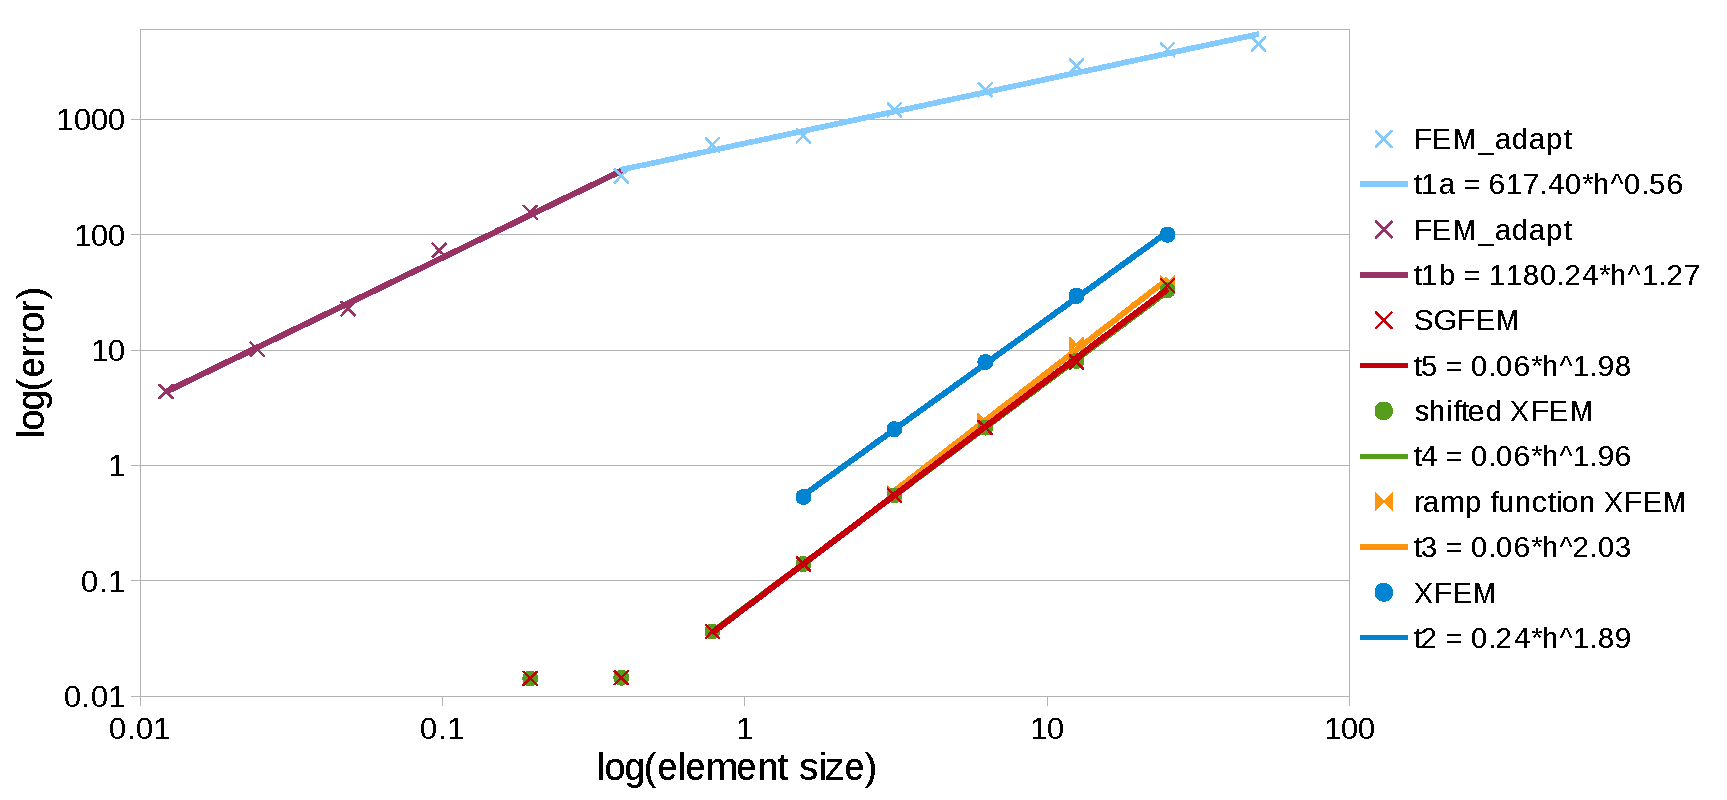
\includegraphics[width=\textwidth]{results/convergence.pdf}
  \caption[Convergence graph \prob{1}]{Convergence graph of different methods on 
  \prob{1}. The error is computed in $L^2$ norm.}
  \label{fig:convergence}
\end{figure}

When solving the \prob{2}, see \fig{fig:convergence_sin}, we plot the convergence graph of the
standard FEM on the problem with the well omitted as a reference (finding only the regular part $u_r$), 
see the 'FEM (ur)' with optimal convergence rate 2.0. The closer the PU methods are to 'FEM (ur)' the better 
the approximation of the singularity is.

In case of the standard FEM we see the same behavior as in \fig{fig:convergence}. The dominant error still 
comes from the singular part of the solution. 

All the PU methods have again nearly optimal convergence rate. The standard XFEM and the ramp function XFEM
are stopped at element size close to 1.0 due to the growth of the condition number of the system matrix.

While decreasing the element size under 1.0, we engage some new kind of error in the shifted XFEM and the 
SGFEM solution. We denied any problems in the adaptive quadrature after several tests -- increasing the number
of refinement levels, using a higher order quadrature. We suspect a bug in our implementation of the well boundary 
integral in \eqref{eqn:weak_form} because the lack of convergence appears right after the well starts to 
intersect more than one element.

\begin{figure}[!htb]
%   \vspace{0pt}
  \centering    
  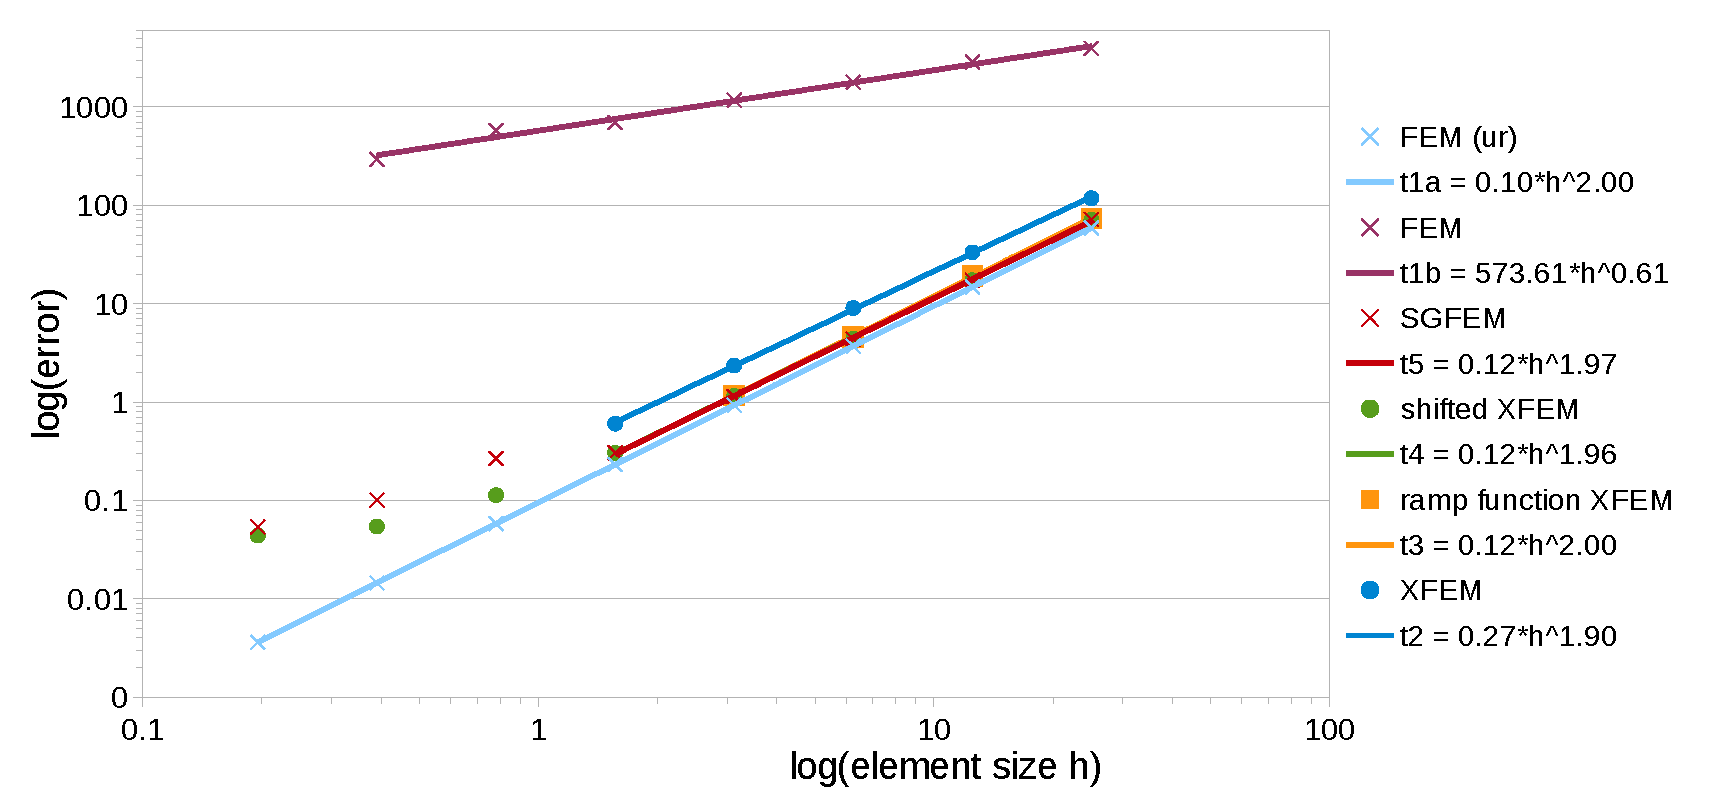
\includegraphics[width=\textwidth]{results/convergence_sin.pdf}
  \caption[Convergence graph \prob{2}]{Convergence graph of different methods on 
  \prob{2} in $L^2$ norm. The 'FEM (ur)'
  data comes from the problem without well solved by classical FEM and with optimal convergence rate 2.0.}
  \label{fig:convergence_sin}
\end{figure}

\subsection{Conditioning of the system matrix} \label{sec:res_conditioning}
We shall write here a brief note about the conditioning of the system as we mentioned problems above when using some of the PU methods. 
Condition number for matrices resulting from conforming FEM applied to Laplace equation is $O(h^{-2})$, so the iteration count 
for CG without preconditioning is $O(h^{-1})=O(\sqrt(n))$, where $n=1/h^2$ is number of degrees of freedom. 
With local preconditioning (Jacobi, 
SOR, ILU) one can usually achieve the number of iterations $O(h^{-0.5})$, c.f. \cite{ern_evaluation_2006}.

Let us use the data from the numerical tests above in \ref{sec:res_comparison}.
We observe the iteration count needed by CG solver and gather the values in the graph in \fig{fig:iterations}.
The number of iterations of the standard FEM is corresponding to the classic results as mentioned in the paragraph above. 

\begin{figure}[!htb]
%   \vspace{0pt}
  \centering    
  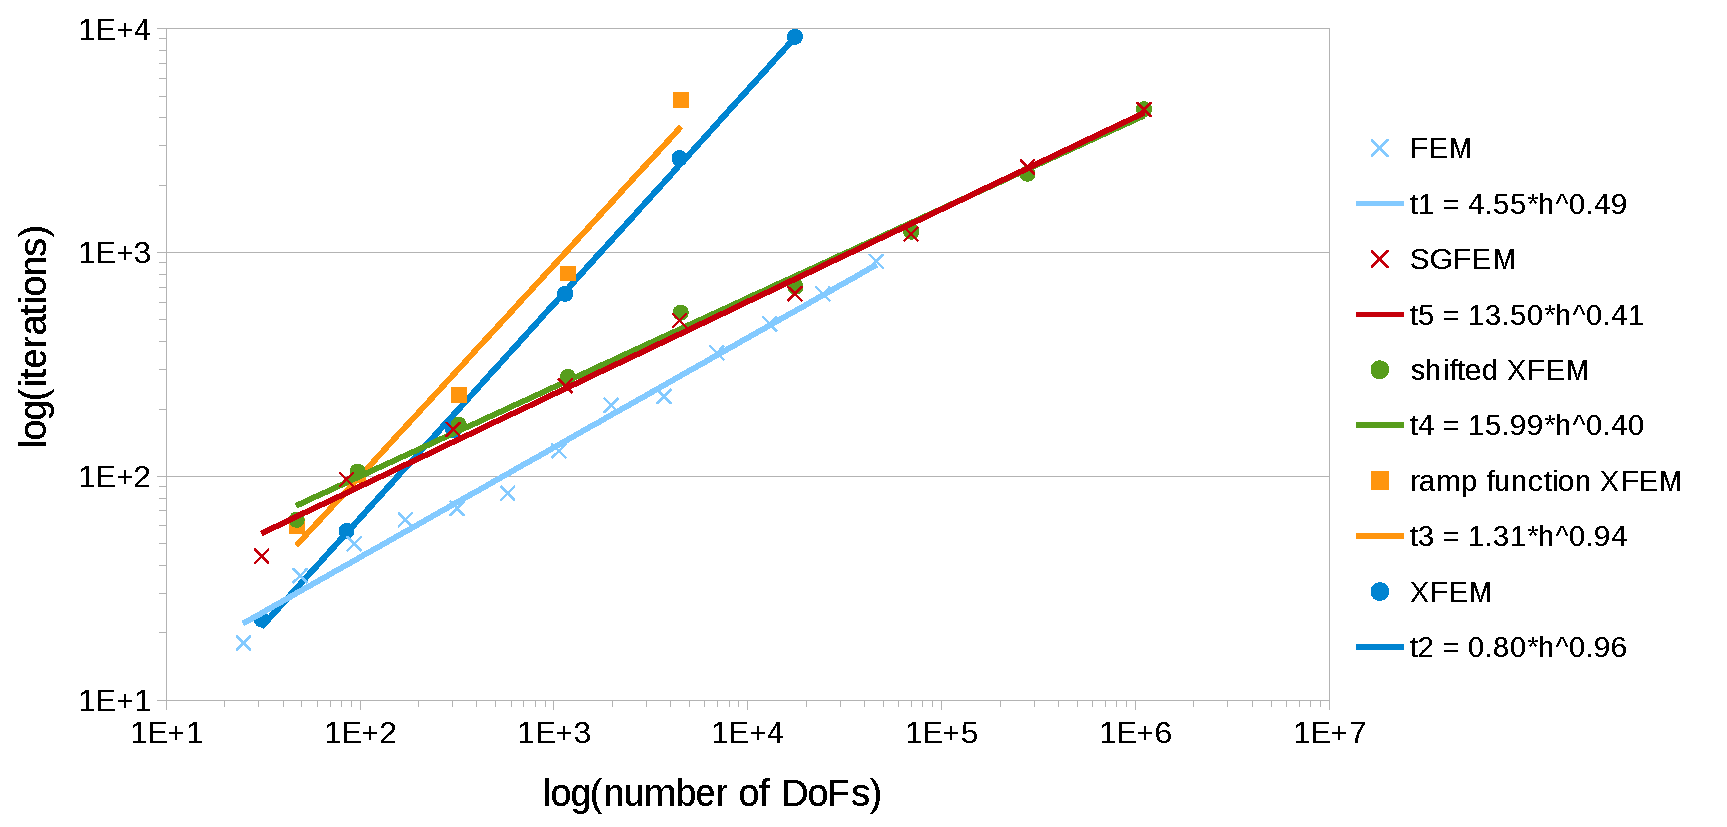
\includegraphics[width=\textwidth]{results/iterations.pdf}
  \caption[Iterations graph]{Graph of dependence of the CG iteration count on the 
  number of degrees of freedom. Measured on both problems with no serious distinction observed.}
  \label{fig:iterations}
\end{figure}
%
We can see clearly the enormous growth of the number of iterations in case of the standard XFEM and the ramp 
function XFEM. These problems are generally known and are described for example in the overview of the XFEM in
\cite{fries_xfem_overview_2010}. The usage of enrichment functions can make the approximation space almost linearly 
dependent from which the ill-conditioning of the system arises. That is exactly what the SGFEM was developed to deal with.

Summarizing the theory in \cite{babuska_stable_2012} we can say that the conditioning of the SGFEM system is not worse than the one of the 
associated standard FEM system. We have only the number of iterations on the standard FEM system for comparison, 
but we see from the graph in \fig{fig:iterations} that the results in case of the SGFEM are satisfying.
CG used on the shifted XFEM system has similarly good results. This area of the problem would need deeper 
investigation and we will look at it in a part of our following work.


\subsection{Dependence on the enrichment radius}
%
\begin{figure}[!htb]
%   \vspace{0pt}
  \centering    
  \subfloat[$\|\log \vc x - u_h\|^2_{H^1(T)}$ in log scale]{\label{fig:log_estimate_a} 
    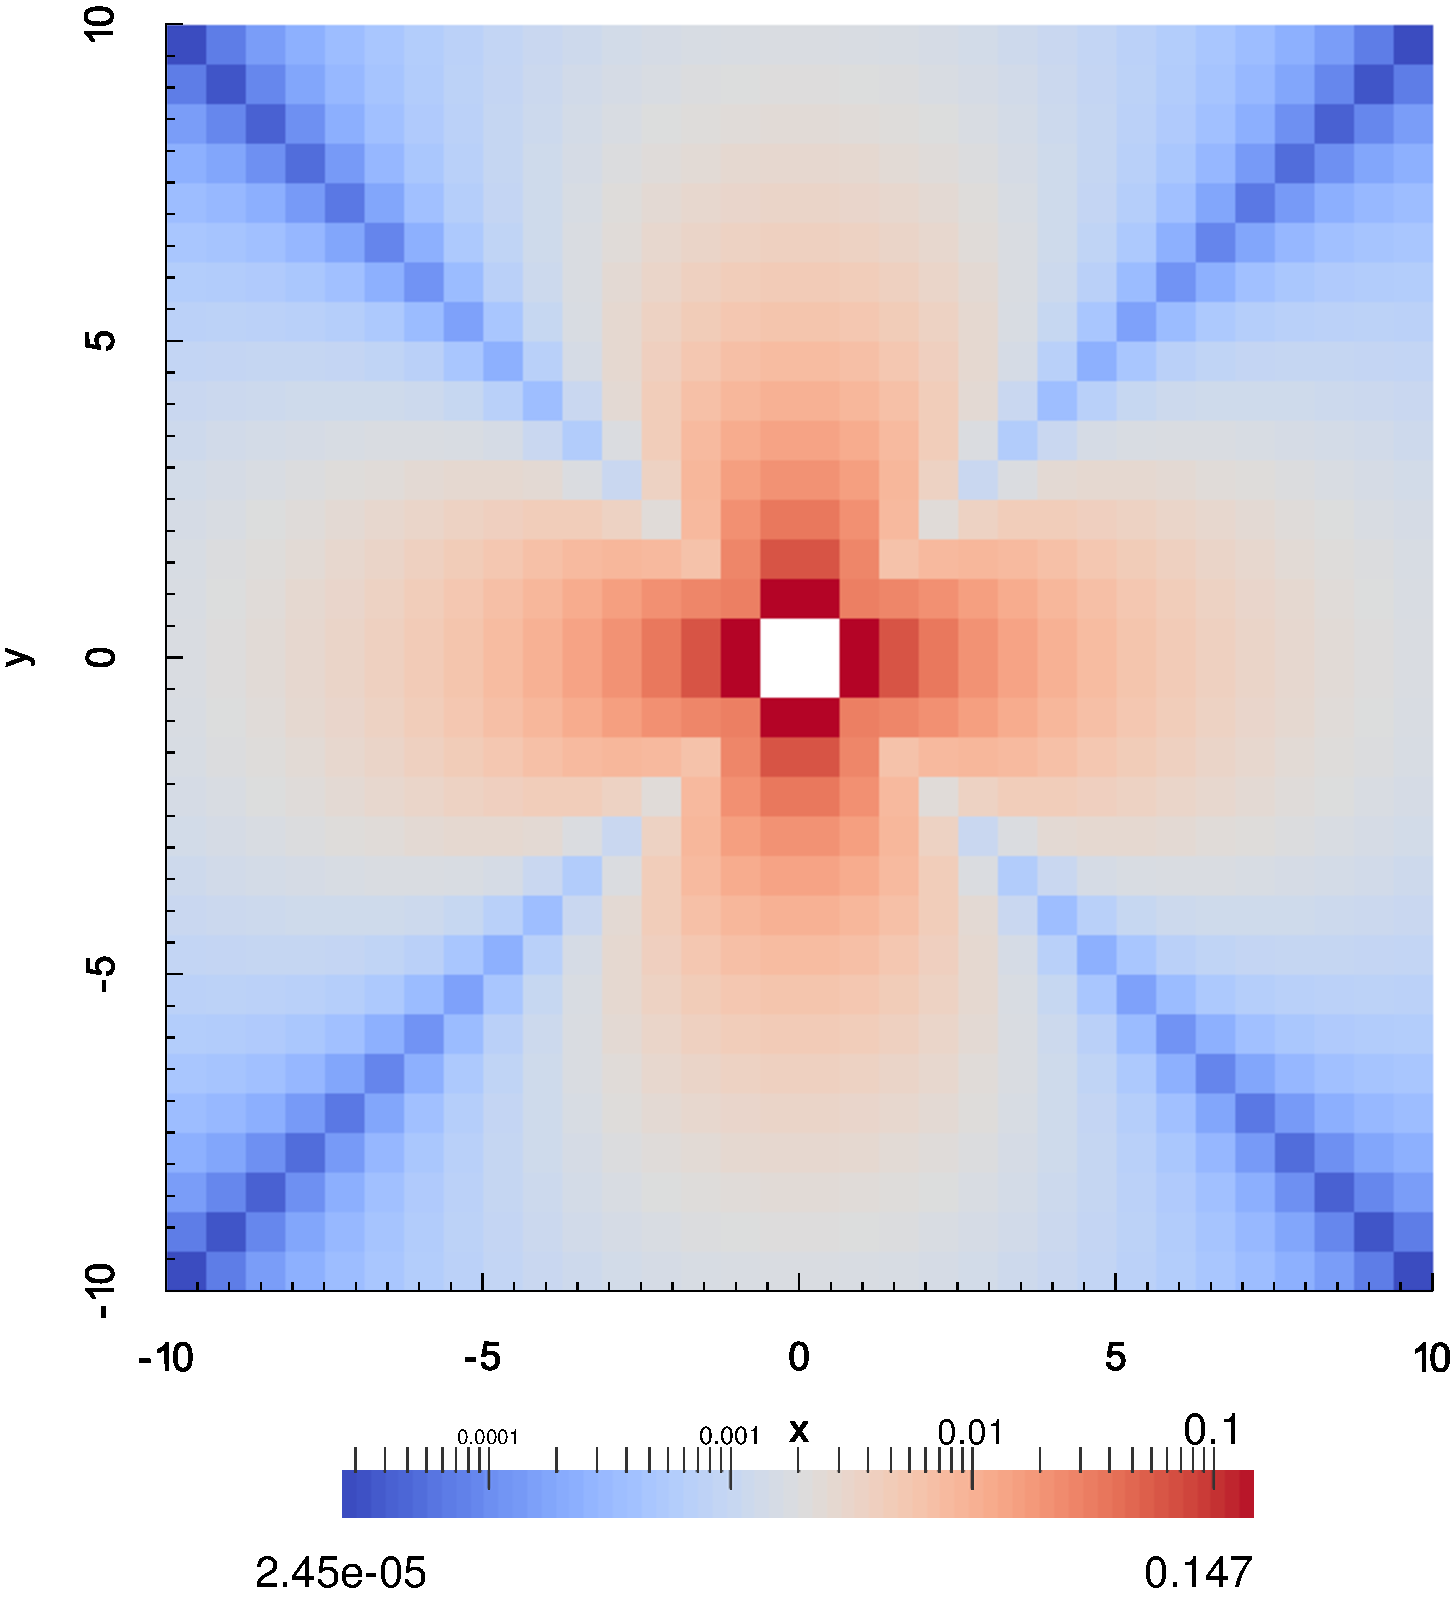
\includegraphics[width=0.47\textwidth]{results/log_estimate_h1.pdf} }
  \hspace{0pt}
  \subfloat[the ratio \eqref{eqn:log_h1_estimate_ratio}]{\label{fig:log_estimate_b} 
    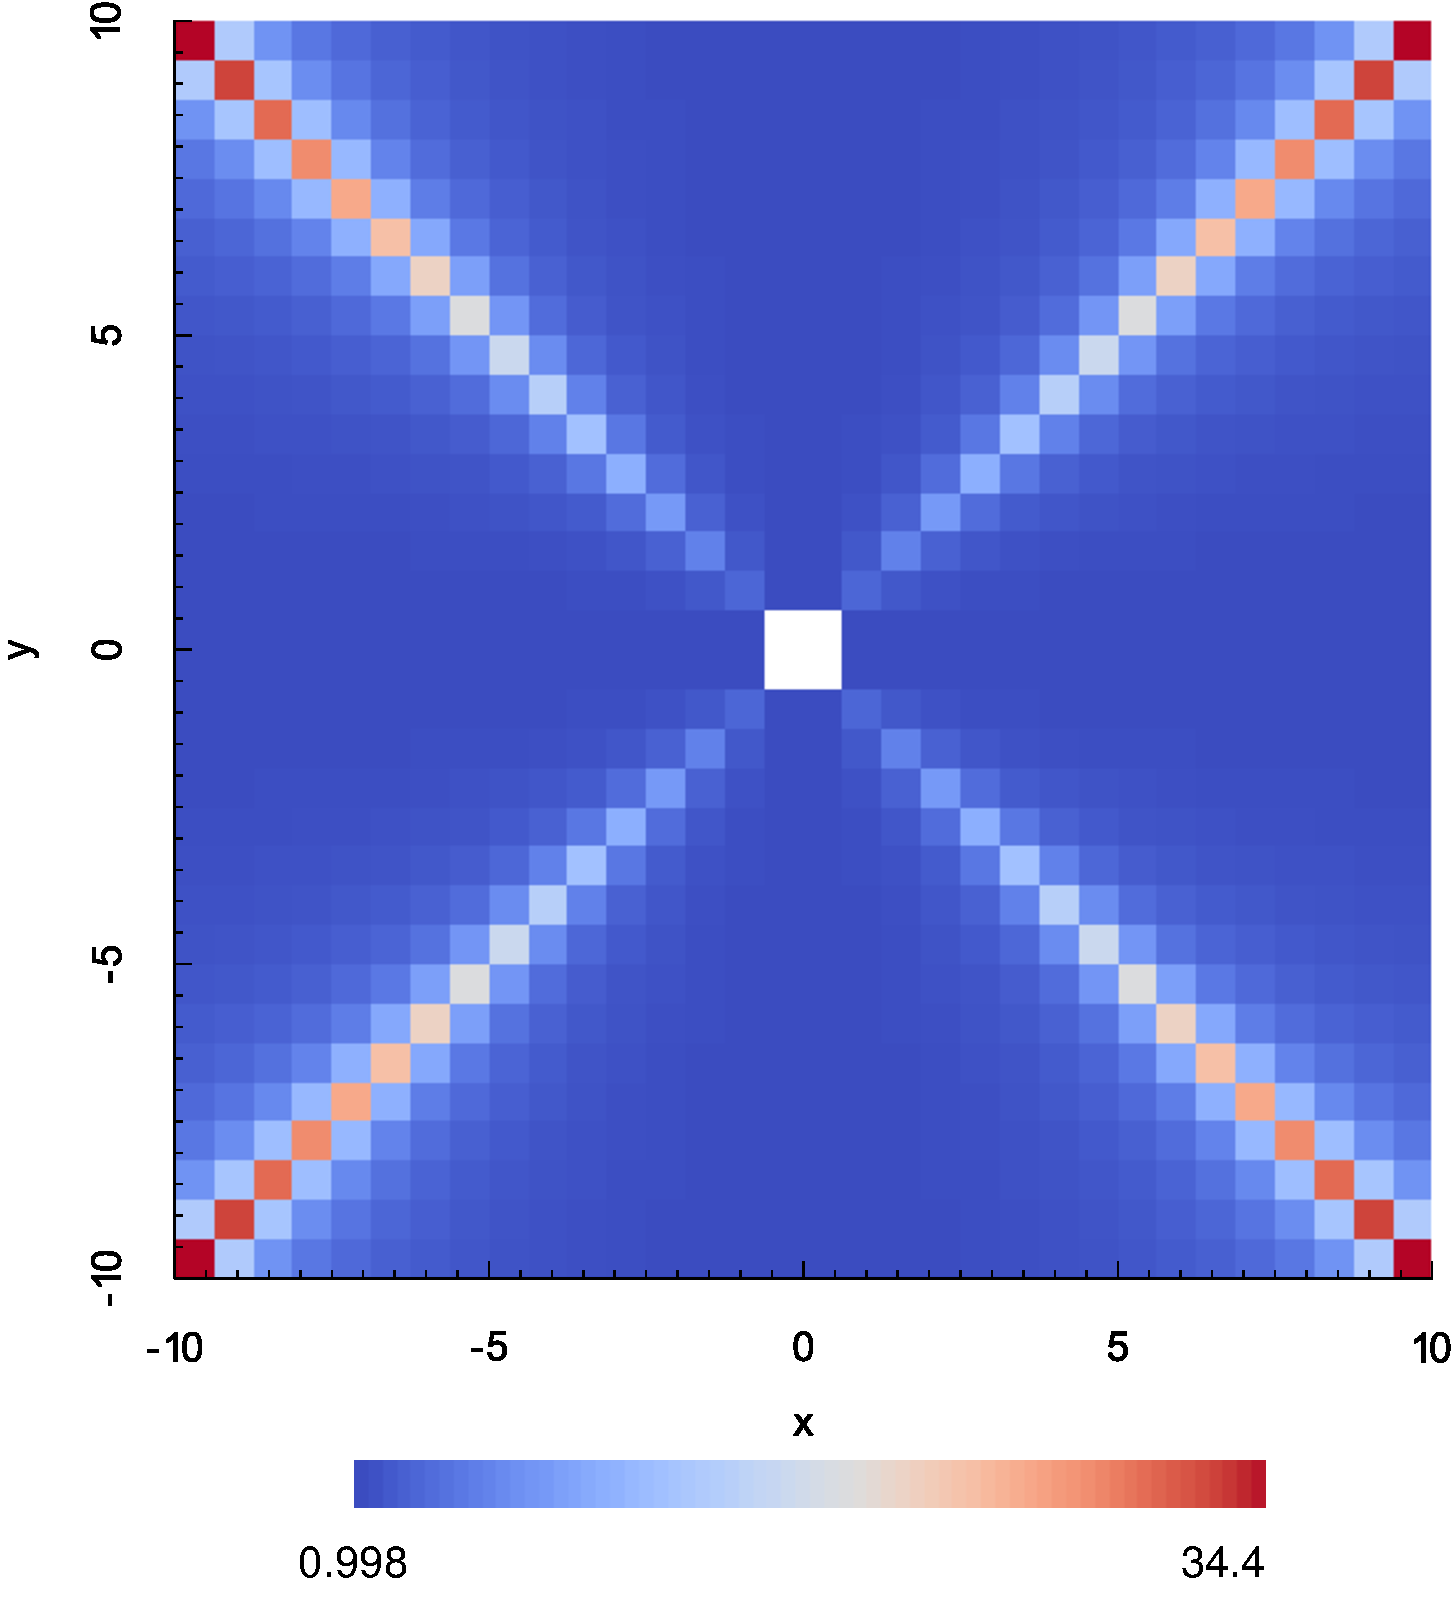
\includegraphics[width=0.47\textwidth]{results/log_estimate_ratio.pdf} }
  \caption[Log error estimate.]
  {
  Results of the numerical validation of the estimate \eqref{eq:grad_estimate_on_square}. The elements are left out 
  in the center where the $\log$ singularity is situated and where the function is cut off.
  }
  \label{fig:log_estimate}
\end{figure}
%
\begin{table}
\begin{center}
\begin{tabular}{crr}
\toprule
% \multicolumn{2}{c}{Item} \\
% \cmidrule(r){1-2}
$h$    & min & max \\
\midrule
$\rfrac{14}{8}$   & 0.97 & 7.1  \\% & 1.38 & 10.0  \\ %& 0.7 & 5.3   \\
$\rfrac{14}{16}$  & 0.99 & 16.4  \\% & 1.40 & 23.1  \\ %& 1.0 & 17.4  \\
$\rfrac{14}{32}$  & 1.00 & 34.4  \\% & 1.41 & 48.7  \\ %& 1.5 & 51.8  \\
$\rfrac{14}{64}$  & 1.00 & 70.3  \\% & 1.41 & 99.5  \\ %& 2.1 & 150   \\
$\rfrac{14}{128}$ & 1.00 (0.756)& 142.0   \\% & 1.41 & 201   \\ %& 3.0 & 427   \\
\bottomrule
\end{tabular}
\caption{Minimal and maximal values of the ratio \eqref{eqn:log_h1_estimate_ratio} for sequence of refined 
meshes with element size $h$. Validation of the estimate \eqref{eq:grad_estimate_on_square}.}
\label{tab:log_h1_estimate}
\end{center}
\end{table}
%
The aim of this section is twofold: we first validate the estimate \eqref{eq:grad_estimate_on_square}, secondly we study 
numerically dependence of $L^2$ norm of the error on the enrichment radius and compare it with \eqref{eq:singular_approx_error}.

Validity of the estimate \eqref{eq:grad_estimate_on_square} is verified by calculation of the ratio
\begin{equation} \label{eqn:log_h1_estimate_ratio}
\frac{h^{3/2} r^{-2} 12^{-1/2}}{\|u_s - \Pi u_s\|^2_{H^1(T)}},\quad u_s(\vc x) = \log \abs{\vc x}
\end{equation}
on every element $T$ of the sequence of refined meshes using a $5\times5$ Gaussian quadrature for estimation of the $H^1$ norm. Table 
\ref{tab:log_h1_estimate} reports the minimum and the maximum value of the ratio over all elements of every mesh.
The minimum value are close to 1 independently of $h$ which is in perfect agreement with \eqref{eq:grad_estimate_on_square}.
Moreover, the minimum value is attained on the majority of
elements, see Figure \fig{fig:log_estimate_b}. Both parts of Figure \fig{fig:log_estimate} demonstrate also higher convergence rate on diagonal elements
where the nonlinear term of the tensor product bilinear finite elements allows better approximation of the saddle shaped logarithmic surface.

Next, we study influence of the enrichment radius $R$ to the global $L^2$ error. To this end, we have run solution of Problem 2 with parameter $U=3$
using shifted XFEM as described in the previous section for different mesh step and different values of $R$.
Let us remind that $O(h^p)$ convergence of the $H^1$ norm translates to the $O(h^{p+1})$ convergence of the $L^2$ norm 
for the linear elliptic problems (c.f. \cite[Theorem 19.2]{ciarlet_basic_1991}). According to the estimates \eqref{eq:std_err_estimate}
and \eqref{eq:singular_approx_error}, we expect $O(h^2)$ convergence of $L^2$ norm independently of the enrichment radius. This is 
clearly demonstrated on Figure \fig{fig:radius_conv_1}. Lack of convergence under certain error threshold is probably due to 
quadrature error as discussed in the previous section. For comparison, we plot also error of the regular part of the solution
\[
  u_r(x,y) = U \sin (\omega x)
\]
]
resolved by unenriched FEM displaying $O(h^2)$ convergence. \noteJB{Is it really $u_r$ what is plotted, make it clear in caption.}
As predicted the total error diminish with $R$ but can not 
drop under the the error of $u_r$. By direct computation, we get
\[
  \norm{u_r - \Pi u_r}_{H^1(\Omega)} = \frac{1}{12}UHh\omega^2 + O(h^2)
\]
where $H=100$ is domain side and $U=3$, $\omega=0.03$. Then according to \eqref{eq:singular_approx_error},
we get critical value of the enrichment radius
\[
    R_c \sim \sqrt{\frac{\pi}{6}} h/\norm{u_r - \Pi u_r}_{H^1(\Omega)} \sim 9.2
\]
This value roughly match a breakpoint on plots of error in dependence of $R$ on 
on Figure \fig{fig:radius_conv_1}.


\begin{figure}[!htb]
%   \vspace{0pt}
  \centering    
  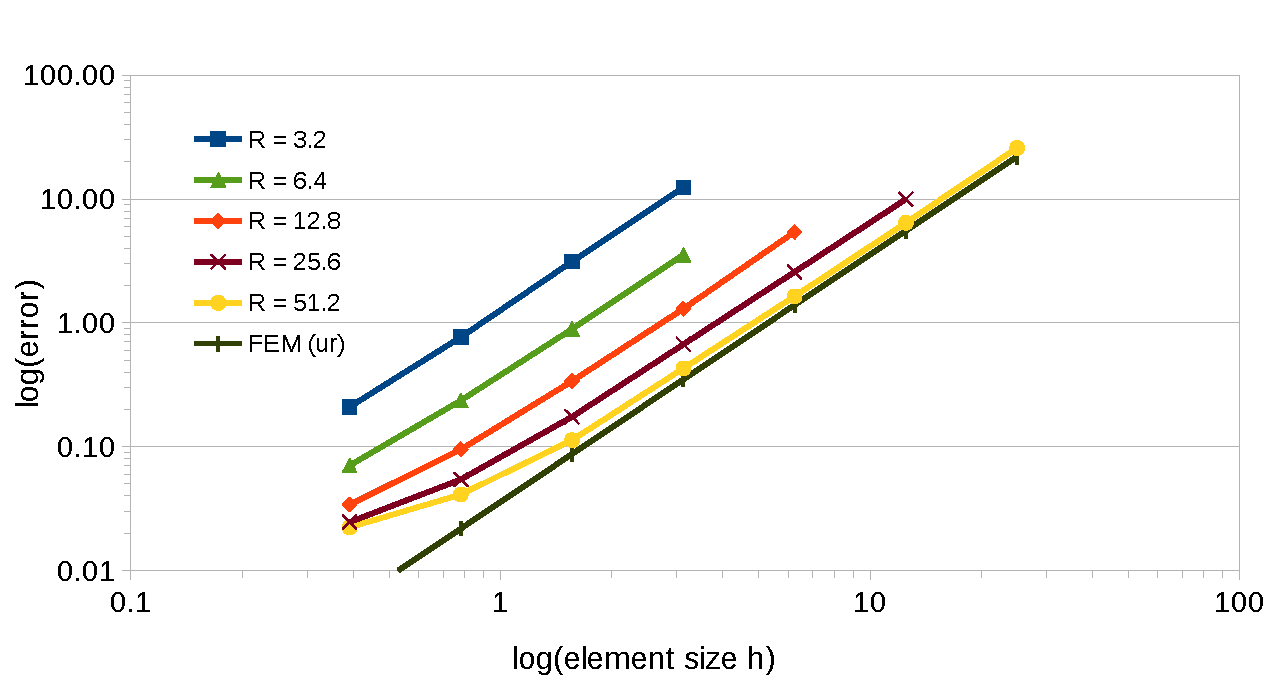
\includegraphics[width=0.9\textwidth]{results/radius_conv_1.pdf}
%   \subfloat[rozdìlený element s vrtem]{\label{fig:adapt_ref_a} 
%     \includegraphics[width=70mm]{\figpath adaptive_ref.pdf} }
%   \hspace{0pt}
%   \subfloat[detail hranice vrtu]{\label{fig:adapt_ref_b} 
%     \includegraphics[width=72mm]{\figpath adaptive_ref_detail.pdf} }
  \caption[Enrichment radius choice.]{Convergence graph for different enrichment radii. The 'FEM (ur)'
  data comes from the problem without well solved by the standard FEM -- it has the optimal convergence rate 2.0.}
  \label{fig:radius_conv_1}
\end{figure}
\begin{figure}[!htb]
%   \vspace{0pt}
  \centering    
  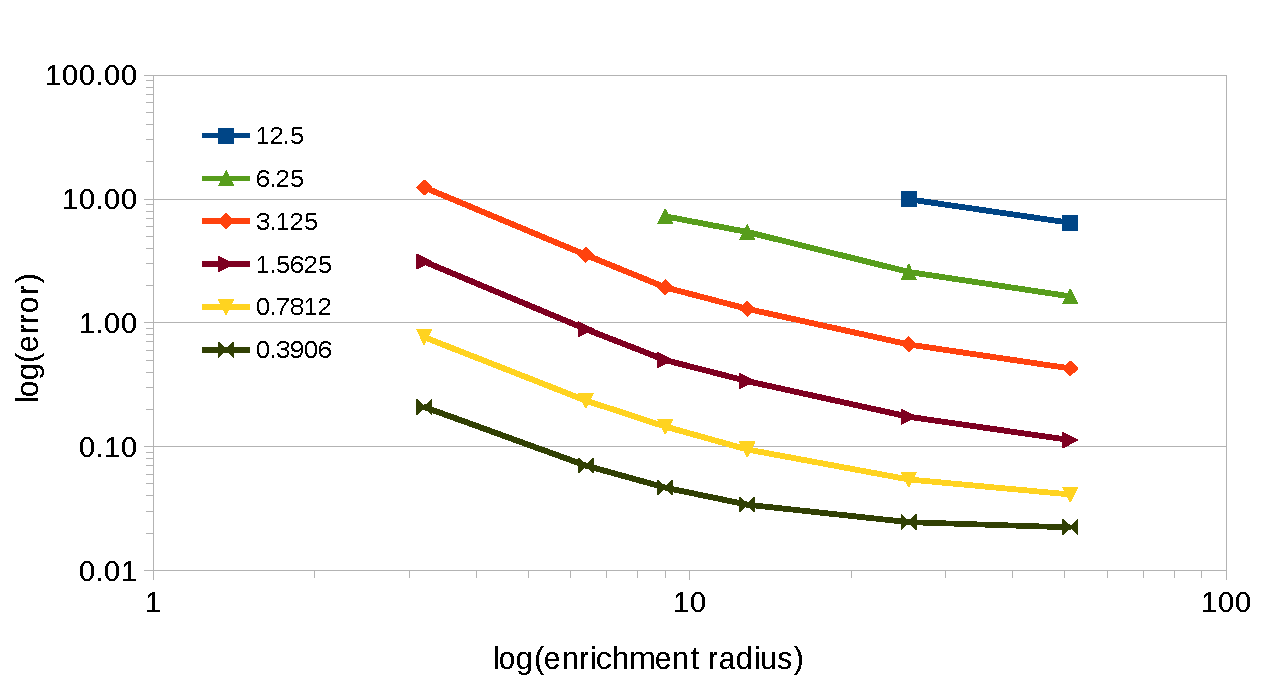
\includegraphics[width=0.9\textwidth]{results/radius_conv_2.pdf}
%   \subfloat[rozdìlený element s vrtem]{\label{fig:adapt_ref_a} 
%     \includegraphics[width=70mm]{\figpath adaptive_ref.pdf} }
%   \hspace{0pt}
%   \subfloat[detail hranice vrtu]{\label{fig:adapt_ref_b} 
%     \includegraphics[width=72mm]{\figpath adaptive_ref_detail.pdf} }
  \caption[Enrichment radius choice.]{Dependence of the error on the enrichment radius for different
  element sizes.}
  \label{fig:radius_conv_2}
\end{figure}





\section{Summary}
\label{sec:summary}

We presented a study on the usage of several PU methods -- the XFEM, its corrected version with the ramp 
function and the shiftment, and the SGFEM. The problem setting was inspired by the work \cite{gracie_modelling_2010,craig_using_2011} 
of R.~Gracie and J.R.~Craig but our effort was aimed more in understanding of the PU methods and their comparison
rather than in computation of complex problems.

We investigated the issue of a sub-optimal convergence rate addressed in \cite{gracie_modelling_2010}. We revealed the problem
in the adaptive quadrature and we suggested better adaptivity rules. The improvement was confirmed by the numerical
tests in \ref{sec:res_comparison} where we obtained optimal convergence rates.

All the implemented methods were compared in \ref{sec:res_comparison}. Regarding the XFEM we saw that at 
least the ramp function must be used in order to obtain optimal convergence. The shifted XFEM and 
the SGFEM converged optimally and did not show any difference in the solution precision.

The ill-conditioning of the system matrix was encountered when using the standard XFEM and the ramp function XFEM.
The iteration count was measured.

From the results in \ref{sec:res_comparison} we saw that the usage of the shifted XFEM or SGFEM 

\section{Acknowledgement}
This work was made under the sincere guidance and support of Mgr. Jan B{\v r}ezina, Ph.D.

This work was supported by the Ministry of Education of the Czech Republic within the SGS project 
no. 21066/115 on the Technical University of Liberec.

%% The Appendices part is started with the command \appendix;
%% appendix sections are then done as normal sections
%% \appendix

%% \section{}
%% \label{}

%% If you have bibdatabase file and want bibtex to generate the
%% bibitems, please use
%%
%%  \bibliographystyle{elsarticle-harv} 
%%  \bibliography{<your bibdatabase>}

%% else use the following coding to input the bibitems directly in the
%% TeX file.

% \begin{thebibliography}{00}
% 
% %% \bibitem[Author(year)]{label}
% %% Text of bibliographic item
% 
% \bibitem[ ()]{}
% 
% \end{thebibliography}
 %\nocite{dip}
 %\bibliographystyle{elsarticle-harv} 
 %\bibliographystyle{elsarticle-num-names} 
 \bibliographystyle{elsarticle-num} 
 \bibliography{../citace.bib}
\end{document}


%\endinput
%%
%% End of file `elsarticle-template-harv.tex'.

